%%%%%%%%%%%%%%%%%%%%%%%%%%%%%%%%%%%%%%%%%
% CLASS OPTIONS
% language: czech/english/slovak
% thesis type: bachelor/master/dissertation
% color: bw for black&white OR no option for default color scheme
% electronic (oneside) or printed (twoside), twoside is default
% paragraph - if passed, this optional argument sets paragraphs as the deepest level of headers, styles it, numbers it and adds it to Table of Content. Use with care! Normally, it is considered unwise to use it, since its too deep.
%%%%%%%%%%%%%%%%%%%%%%%%%%%%%%%%%%%%%%%%%
\PassOptionsToPackage{table}{xcolor}
\documentclass[english,bachelor,unicode,oneside]{ctufit-thesis}

\ctufittitle{Project Adaptation in Code Completion via In-Context Learning}
\ctufitauthorfull{Maksim Sapronov}
\ctufitauthorsurnames{Sapronov}
\ctufitauthorgivennames{Maksim}
\ctufitsupervisor{Evgenii Glukhov, M.Sc.}
\ctufitdepartment{Department of Applied Mathematics}
\ctufityear{2025}
\ctufitdeclarationplace{Prague}
\ctufitdeclarationdate{\today}
\ctufitabstractENG{This thesis addresses the challenge of enhancing code completion models with repository-level context awareness. Modern completion systems struggle with information dispersed across large codebases, limiting their performance. The work presents a context composition framework that extracts relevant repository information and a fine-tuning pipeline for model adaptation, evaluated through systematic experimentation. The research demonstrates that context selection strategy significantly impacts completion quality during inference, while repository-level pre-training preserves in-context learning capabilities. Notably, the study demonstrates that computational requirements for context window extension can be substantially reduced while maintaining competitive performance, advancing code completion by enabling better integration of project-wide information.\blfootnote{Home page: \url{https://github.com/sapromak/adaptive-code-completion}}}
\ctufitkeywordsENG{repository-level code completion, project adaptation, in-context learning, long context, context extension, resource efficiency, Transformer, Code LLM}
\ctufitabstractCZE{Tato bakalářská práce se zabývá problematikou vylepšení modelů pro dokončování kódu s povědomím o kontextu na úrovni repozitáře. Moderní systémy pro dokončování kódu mají potíže s informacemi rozptýlenými napříč rozsáhlými kódovými základnami, což omezuje jejich výkonnost. Práce představuje framework pro kompozici kontextu, který extrahuje relevantní informace z repozitářů, a pipeline pro dolaďování modelů, hodnocené prostřednictvím systematického experimentování. Výzkum ukazuje, že strategie výběru kontextu významně ovlivňuje kvalitu dokončování během inference, zatímco předtrénování na úrovni repozitáře zachovává schopnosti učení v \mbox{kontextu}. Studie zejména prokazuje, že výpočetní požadavky pro rozšíření kontextového okna lze výrazně snížit při zachování konkurenceschopného výkonu, čímž posouvá dokončování kódu vpřed umožněním lepší integrace \mbox{informací} v rámci celého projektu.\blfootnote{Domovská stránka: \url{https://github.com/sapromak/adaptive-code-completion}}}
\ctufitkeywordsCZE{dokončování kódu na úrovni repozitáře, projektové přizpůsobení, učení v kontextu, dlouhý kontext, rozšíření kontextu, účinné využívání zdrojů, Transformer, Code LLM}

%%%%%%%%%%%%%%%%%%%%%%%%%%%%%%%%%%
% CUSTOMIZATION of this template
% Skip this part or alter it if you know what you are doing.
%%%%%%%%%%%%%%%%%%%%%%%%%%%%%%%%%%

\RequirePackage{iftex}[2020/03/06]
\iftutex % XeLaTeX and LuaLaTeX
    \RequirePackage{ellipsis}[2020/05/22] % ellipsis workaround for XeLaTeX
\else
    \errmessage{Only compilation with XeLaTeX or LuaLaTeX is allowed}
    \stop
\fi

% hyperlinks
\hypersetup{
    pdfpagelayout=TwoPageRight,
    colorlinks=false,
    allcolors=decoration,
    pdfborder={0 0 0.1}
}

% uncomment the following to change the color of all hyperlinks to CTU blue
%\hypersetup{allbordercolors=decoration}

\RequirePackage{pdfpages}[2020/01/28]

%%%%%%%%%%%%%%%%%%%%%%%%%%%%%%%%%%
% CUSTOMIZATION of this template END
%%%%%%%%%%%%%%%%%%%%%%%%%%%%%%%%%%


%%%%%%%%%%%%%%%%%%%%%%
% DEMO CONTENTS SETTINGS
%%%%%%%%%%%%%%%%%%%%%%
\usepackage{dirtree}
\usepackage{lipsum,tikz}
\usepackage[style=iso-authoryear,backend=biber,uniquename=false,uniquelist=false,sorting=nyt]{biblatex}
\addbibresource{text/bib-database.bib}
\usepackage{array}
\usepackage{xurl}
\usepackage{listings}
\usepackage{minted}
\usepackage{csquotes}
\usepackage{bm}
\usepackage{commath}
\usepackage{fontspec}
\usepackage{etoolbox}
\usepackage{soul}
\usepackage{xspace}
\usepackage{graphicx}
\usepackage{booktabs}
\usepackage{multicol}
\usepackage{multirow}
\usepackage{makecell}
\usepackage[table]{xcolor}
\usepackage{paralist}
\usepackage{tcolorbox}
\usepackage{float}
\usepackage{adjustbox}
\usepackage{pgfplots}
\usepackage{bbding}
\usepackage{nameref}
\usepackage{hyperref}

\DefineBibliographyStrings{english}{
  andothers = {et~al.}
}
\renewcommand*{\nameyeardelim}{\hspace{0.35em}}
\let\familynameformat=\relax
\ExecuteBibliographyOptions{maxcitenames=1,mincitenames=1}

% Create a separate category for self-citing
\DeclareBibliographyCategory{our_papers}
\addtocategory{our_papers}{sapronov2025}

% Add this to define \citet command using biblatex functionality with clickable author names
\DeclareCiteCommand{\citet}
  {\usebibmacro{prenote}}
  {\usebibmacro{citeindex}%
   \bibhyperref{%
     \printnames{labelname}%
     \setunit{\printdelim{nameyeardelim}}%
     \printtext[parens]{\usebibmacro{cite:labeldate+extradate}}%
   }}
  {\multicitedelim}
  {\usebibmacro{postnote}}

% Add this configuration to make the entire citation a hyperlink
\ExecuteBibliographyOptions{hyperref=true}
\DeclareFieldFormat{citehyperref}{%
  \bibhyperref{#1}}
\DeclareFieldFormat{textcitehyperref}{%
  \bibhyperref{#1}}
\DeclareFieldFormat{citesetup}{%
  \bibhyperref{#1}}
\DeclareFieldFormat{parencite}{%
  \bibhyperref{\mkbibparens{#1}}}

% For name+year citations
\letbibmacro{cite:labelyear+extrayear}{cite:labeldate+extradate}
\renewbibmacro*{cite}{%
  \printtext[citehyperref]{%
    \printnames{labelname}%
    \setunit{\printdelim{nameyeardelim}}%
    \usebibmacro{cite:labeldate+extradate}}}

\renewbibmacro*{textcite}{%
  \printtext[textcitehyperref]{%
    \printnames{labelname}%
    \setunit{\printdelim{nameyeardelim}}%
    \usebibmacro{cite:labeldate+extradate}}}

\DeclareCiteCommand{\citeyear}
    {}
    {\bibhyperref{\printdate}}
    {\multicitedelim}
    {}

\newfontface\lserif{Liberation Serif}

\newcommand{\Csh}{C{\lserif\#}}
\newcommand{\chapterref}[1]{\hyperref[#1]{Chapter~\ref*{#1}}}
\newcommand{\sectionref}[1]{\hyperref[#1]{Section~\ref*{#1}}}
\newcommand{\figureref}[1]{\hyperref[#1]{Figure~\ref*{#1}}}
\newcommand{\tableref}[1]{\hyperref[#1]{Table~\ref*{#1}}}
\newcommand{\equationref}[1]{\hyperref[#1]{Equation~\ref*{#1}}}
\newcommand{\appendixref}[1]{\hyperref[#1]{Appendix~\ref*{#1}}}
\newcommand{\shortcaption}[2]{\caption[#1]{#2}}

\newcommand\blfootnote[1]{%
  \begingroup
  \renewcommand\thefootnote{}\footnote{#1}%
  \addtocounter{footnote}{-1}%
  \endgroup
}

%%%%%%%%%%%%%%%%%%%%%%
% DEMO CONTENTS SETTINGS END
%%%%%%%%%%%%%%%%%%%%%%

\begin{document}
\frontmatter\frontmatterinit

\thispagestyle{empty}\maketitle\thispagestyle{empty}\cleardoublepage

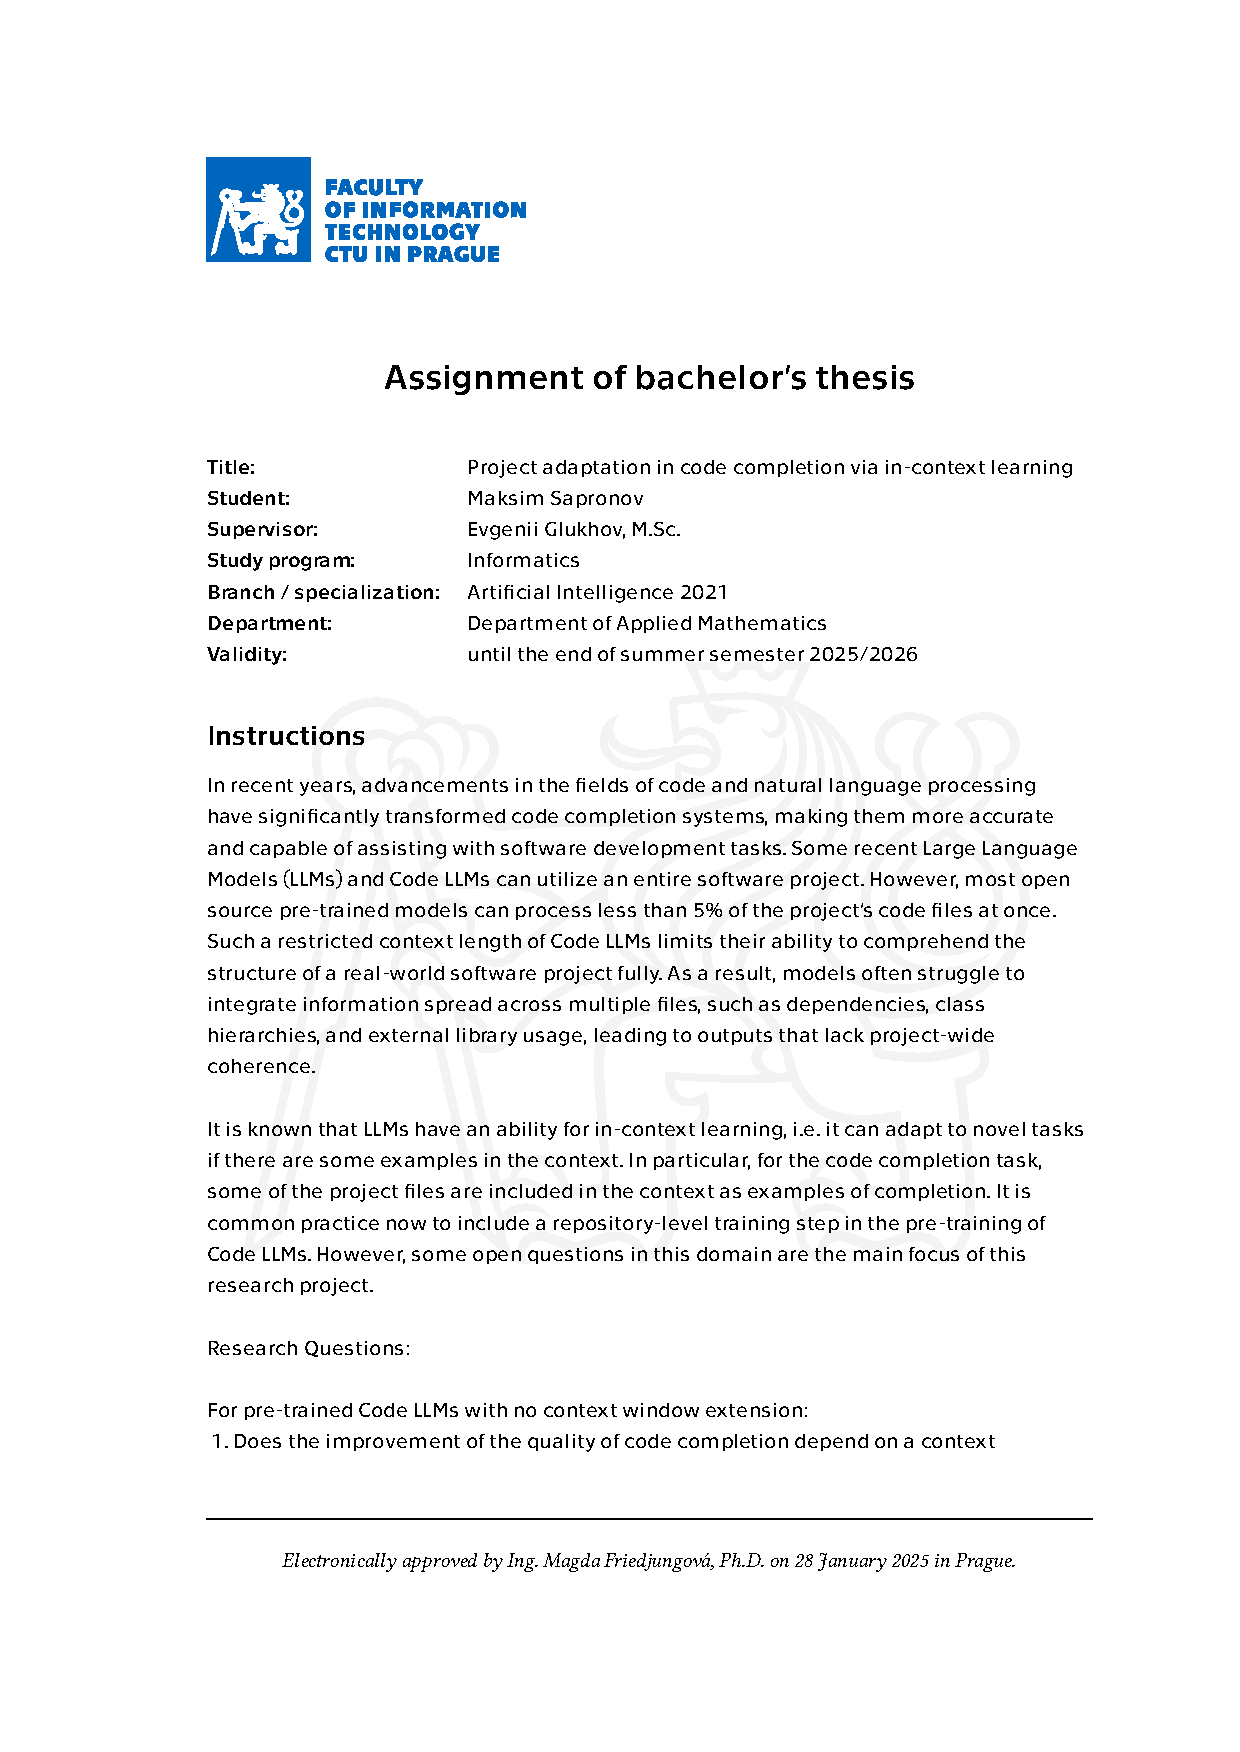
\includepdf[pages={1-}]{assignment.pdf}

\imprintpage
\stopTOCentries
%%%%%%%%%%%%%%%%%%%%%%
% list of other contents END
%%%%%%%%%%%%%%%%%%%%%%

\begin{acknowledgmentpage}
  I would like to express my sincere gratitude to my supervisor, Evgenii Glukhov, M.Sc., whose guidance and advice proved invaluable throughout the preparation of this thesis. I also wish to extend my appreciation to the \mbox{JetBrains} Research association for initiating and supporting this research project by providing both high-level expertise and essential resources. In particular, Alexander Bezzubov, Egor Bogomolov, Timofey Bryksin, and Yaroslav Golubev made \mbox{significant} contributions by advancing a portion of the project to the ICLR 2025 Conference and offering valuable \mbox{feedback} on the paper derived from this thesis. Finally, I am deeply grateful to my family and friends for their \mbox{unwavering} patience and support.
\end{acknowledgmentpage}

% Source of the two first paragraphs: https://courses.fit.cvut.cz/SFE/download/index.html#_documents (document Declaration for FT in English); "authorization" is used instead of "authorisation" and "license" instead of "licence"
\begin{declarationpage}
  I hereby declare that the presented thesis is my own work and that I have cited all sources of information in accordance with the Guideline for adhering to ethical principles when elaborating an academic final thesis.

  I acknowledge that my thesis is subject to the rights and obligations stipulated by the Act No. 121/2000 Coll., the Copyright Act, as amended. In accordance with Section 2373(2) of Act No. 89/2012 Coll., the Civil Code, as amended, I hereby grant a non-exclusive authorization (license) to utilize this thesis, including all computer programs that are part of it or attached to it and all documentation thereof (hereinafter collectively referred to as the ``Work''), to any and all persons who wish to use the Work. Such persons are entitled to use the Work in any manner that does not diminish the value of the Work and for any purpose (including use for profit). This authorization is unlimited in time, territory and quantity.

  I declare that I have used AI tools during the preparation and writing of my thesis. I have verified the generated content. I confirm that I am aware that I am fully responsible for the content of the thesis.
\end{declarationpage}

\newcommand{\printczechabstractpage}{%
\begin{abstractpage}
\begin{abstrakt}%
\begin{sloppypar}\noindent
\thectufitabstrakt
\end{sloppypar}
\end{abstrakt}

\vskip 0.5cm

{\noindent\color{heading}\bfseries Klíčová slova\hspace{1em}}{\thectufitklicovaslova}
\end{abstractpage}
\cleardoublepage
}

\begin{abstractpage}
\begin{abstract}%
\thectufitabstract
\end{abstract}

\vskip 0.5cm

{\noindent\color{heading}\bfseries Keywords\hspace{1em}}{\thectufitkeywords}
\end{abstractpage}
\cleardoublepage

\printczechabstractpage

\tableofcontents
%%%%%%%%%%%%%%%%%%%%%%
% list of other contents: figures, tables, code listings, algorithms, etc.
%%%%%%%%%%%%%%%%%%%%%%
\listoffigures % list of figures
\begingroup
\clearpage
\listoftables % list of tables
\endgroup

\chapter{\thectufitabbreviationlabel}

\begin{tabular}{rl}
  ABF & Adjustment of the Base Frequency\\
  API & Application Programming Interface\\
  Adam & Adaptive Moment Estimation\\
  BPE & Byte Pair Encoding\\
  CE & Cross-Entropy\\
  Code LLM & Code Large Language Model\\
  EM & Exact Match\\
  EOS & End of Sequence\\
  ES & Edit Similarity\\
  FIM & Fill-in-the-Middle\\
  FL & File-Level\\
  GPU & Graphics Processing Unit\\
  ICL & In-Context Learning\\
  IoU & Intersection over Union\\
  LCA & Long Code Arena\\
  LLM & Large Language Model\\
  LM & Language Modeling\\
  MLP & Multi-Layer Perceptron\\
  OOV & Out-of-Vocabulary\\
  Or & Original\\
  PD & Path Distance\\
  PPL & Perplexity\\
  RAG & Retrieval-Augmented Generation\\
  RoPE & Rotational Position Embedding\\
\end{tabular}

\resumeTOCentries
\mainmatter\mainmatterinit
%%%%%%%%%%%%%%%%%%%
% THE THESIS
% MODIFY ANYTHING BELOW THIS LINE
%%%%%%%%%%%%%%%%%%%

\chapter*{Introduction}\addcontentsline{toc}{chapter}{Introduction}\markboth{Introduction}{Introduction}

Software development plays a pivotal role in shaping the modern digital world. Assisting developers in writing code more efficiently has the potential to accelerate innovation across industries by reducing the cognitive and temporal overhead of programming. Over the decades, numerous tools have emerged to support developers, including high-level programming languages, integrated development environments (IDEs), version control systems, and, more recently, AI-powered code assistance. Tasks such as code completion, generation, refactoring, and bug localization are increasingly addressed using Large Language Models (LLMs), which have demonstrated strong capabilities in natural language and code understanding.

Code completion, in particular, benefits significantly from the in-context learning capabilities of LLMs — where the model leverages examples or relevant information provided in the input context to improve predictions without parameter updates. However, while LLMs have advanced in modeling local contexts, a critical limitation remains: their restricted ability to integrate and reason over information dispersed across large codebases. This includes understanding dependencies between files, class hierarchies, and interactions with external libraries — information that is often essential for generating coherent and accurate completions.

Despite the emergence of code-specific LLMs and efforts to incorporate repository-level context during training or inference, most pre-trained models still struggle to process more than a small fraction of a project's code files at once. As a result, they fall short in capturing project-wide structure, leading to incomplete or inaccurate predictions. Therefore, there is a need for continued research within the community developing such models to address these limitations. This thesis focuses on exploring how the composition and organization of contextual information influence the performance of code completion models, particularly in repository-level settings where code is distributed across multiple interdependent files. It investigates how context selection strategies and model adaptations can enhance the ability of pre-trained Code LLMs to generate coherent and accurate completions that reflect the structure and semantics of entire software projects.

% TODO: highlight the novelty of the work
% TODO: references?
% TODO: fill in the structure of the thesis here (w/ or w/o the example list)
% \begin{description}
    % \item[Chapter 1] Description of the first chapter.
    % \item[Chapter 2] Description of the second chapter.
% \end{description}

\chapter*{Objectives of the Thesis}\addcontentsline{toc}{chapter}{Objectives of the Thesis}\markboth{Objectives of the Thesis}{Objectives of the Thesis}

The objectives of this thesis are divided into two parts, corresponding to the theoretical and practical aspects of the work.

The theoretical part aims to provide a comprehensive survey of the challenges associated with project adaptation in the context of full line code completion, focusing on the current capabilities and limitations of in-context learning and repository-level code completion methods. This part establishes the necessary background to understand the practical contributions of the thesis.

The practical part addresses several research questions concerning the impact of various context composition strategies on the quality of code completion, evaluated across three setups: a pre-trained Code Large Language Model (Code LLM), the same model fine-tuned with a specific context composition strategy, and the model after context window extension. To address these questions, the thesis implements a context composition framework for extracting relevant information from software repositories, as well as a fine-tuning pipeline for adapting Code LLMs to project-specific data. The outcomes characterize the role of context composition in enhancing code completion quality and provide insights into its integration within repository-level training procedures.

\part{Conceptual Framework}\label{part:conceptual-framework}  % other options are Theoretical Background, Theoretical Part, Foundational Concepts
\chapter{Code Completion}\label{chap:code-completion}

The upcoming chapter provides a comprehensive examination of code completion. It begins with a definition of the task. The chapter then delves into the motivations for advancing code completion techniques, highlighting their impact on productivity and learning. A historical overview of the evolution of code completion methods is presented, tracing the transition from deterministic approaches to sophisticated learning-based systems. Finally, the chapter categorizes code completion based on various criteria.

\section{Task Definition}
% Relevant papers: bhoopchand2016, ginzberg2017, husein2025, izadi2024, wang2021, ciniselli2021, hindle2012, izadi2022, lu2021

Code completion, also called code suggestion or autocompletion, is a functionality within integrated development environments that enables developers to utilize an automated continuation of the code they are writing. Typically, it is invoked by a trigger model, which aims to anticipate the user's requirement for this functionality. The point of this invocation, whether it is referenced as temporal or spatial, is called a trigger point.

In this work, code completion is regarded as a task rather than a feature, as this perspective highlights the task-methodology relationship and emphasizes the technical aspects over marketing considerations. In addition, the term \textit{completion} is used as a shorthand throughout the text.

\section{Motivation}
% Relevant papers: peng2023, weber2024, bakal2025, takerngsaksiri2023, giagnorio2025

The task of code completion is a pivotal component of contemporary software development, offering substantial benefits that enhance both the productivity and efficiency of developers. This section elucidates the motivations for investigating this task and advancing existing solutions.

By reducing the amount of typing required, code completion allows developers to focus more on the logic and structure of their code rather than the syntax. Studies have shown that AI-powered code completion tools can significantly reduce task execution times, with some reporting up to a 55.8\% reduction in controlled experiments \parencite{peng2023}. These tools also significantly impact developer productivity by reducing the cognitive load associated with coding tasks, achieved through contextually relevant suggestions that streamline the coding process \parencite{weber2024}. Furthermore, the integration of AI in code completion tools has been linked to increased developer satisfaction and efficiency, as it allows developers to complete tasks more swiftly and with greater accuracy \parencite{bakal2025}.

For students and novice programmers, code completion tools serve as a valuable learning aid. They provide real-time feedback and suggestions, helping learners understand programming concepts and syntax more effectively. This educational aspect is highlighted in studies where students reported enhanced learning experiences and increased confidence in their coding abilities \parencite{takerngsaksiri2023}. Moreover, code completion tools provide accurate suggestions that help reduce typo errors and other common mistakes. This is particularly beneficial for new developers or those working with unfamiliar codebases, as it helps them adhere to coding standards and best practices.

Recent advancements in deep learning have enabled the personalization of code completion tools, allowing them to adapt to specific organizational or individual coding styles. This personalization not only improves the relevance of suggestions but also enhances the overall user experience, making these tools more effective and user-friendly \parencite{giagnorio2025}.

Due to the simple and atomic formulation of code completion, it possesses the important property of being fundamental to other AI-powered code assistance features. For instance, code generation can be viewed as a specific extension of code completion, and code editing is a sequence of code generations. This implies that most enhancements achieved through code completion research propagate further, adding new layers of improvements in the field.

In summary, code completion stands as a foundational and multifaceted tool within modern software development. Its benefits extend beyond mere convenience, offering measurable improvements in efficiency, learning, and code quality. As advancements in AI continue to refine its capabilities, code completion not only streamlines day-to-day programming tasks but also acts as a cornerstone for broader innovations in AI-assisted software engineering.

\section{Evolution of Methods}\label{sec:evolution-of-code-completion}
% Relevant papers: mandelin2005, hill2004, han2009, hindle2012, raychev2014, asaduzzaman2014, proksch2015, nguyen2015, bielik2016, ginzberg2017, karampatsis2019, liu2020, alon2019, svyatkovskiy2020, kim2021

\begin{sloppypar}
Approaches to code completion have evolved considerably over the past few decades, progressing from simple deterministic methods to sophisticated learning-based systems. This section highlights key developments in the history of code completion. The Related Work section of the~\citet{ciniselli2021} was mainly used to compile this valuable information.
\end{sloppypar}

In the early years, code completion methods primarily relied on rule-based approaches and static type information. These systems typically presented the user with a list of type-compatible methods or variables, often sorted alphabetically~\parencite{mandelin2005}. While straightforward to implement, these methods lacked contextual awareness and often produced lengthy suggestion lists that were cumbersome to navigate.

A significant advancement came with clone-based completion methods, where code fragments from existing repositories were identified and reused as completion suggestions \parencite{hill2004}. These approaches recognized that developers often write repetitive code patterns, but they were limited by the need for exact or near-exact matches in the code database.

The next major evolution occurred when researchers began applying statistical methods to code completion. \citet{han2009} introduced a novel approach that expanded abbreviated inputs into complete code tokens using Hidden Markov Models trained on example code. This represented an early step toward probabilistic code completion. \citet{hindle2012} demonstrated that software exhibits natural patterns that can be captured by statistical language models, laying the groundwork for treating code completion as a language modeling problem.

Building on this foundation, more sophisticated probabilistic models were developed. \citet{raychev2014} applied statistical language models specifically for code completion tasks, while \citet{bielik2016} introduced probabilistic higher order grammar (PHOG), which parameterized grammar production rules on a context obtained from executing functions learned from data. Bayesian networks were also explored by \citet{proksch2015}, who used additional context information beyond just the static type to generate completion suggestions.

Context-sensitivity became increasingly important as code completion systems matured. \citet{asaduzzaman2014} developed CSCC, which leveraged previous code examples to recommend method calls by considering the surrounding code context. This approach demonstrated how incorporating more contextual information affects the relevance of completion suggestions.

\begin{sloppypar}
The rise of deep learning brought another paradigm shift to code completion. Recurrent neural networks (RNNs), particularly long short-term memory (LSTM) networks, were applied to model the sequential nature of code. \citet{ginzberg2017} explored both standard LSTMs and attention-augmented networks for token-level code completion, establishing new capabilities in code prediction tasks.
\end{sloppypar}

Recent years have witnessed the adoption of even more powerful neural architectures. \citet{karampatsis2019} tackled the out-of-vocabulary problem in code completion using subword units with neural language models. \citet{liu2020} leveraged multi-task learning and pre-trained language models for code completion, while also incorporating type information to assist in identifier prediction.

The latest advancements utilize transformer-based architectures, which have proven effective in natural language processing (NLP). \citet{svyatkovskiy2020} introduced IntelliCode Compose, a general-purpose code completion tool that predicts sequences of code tokens using a transformer model. \citet{kim2021} enhanced transformer models by incorporating syntactic structure awareness through abstract syntax tree (AST)-based representations. These transformer architectures address limitations of previous sequence models by allowing attention to any part of the input context, rather than relying solely on sequential information. Furthermore, attention mechanisms enable transformers to consider relationships between distant parts of the code that have semantic connections, overcoming the long-range dependency challenges faced by RNN-based approaches.

Parallel to these developments, structural approaches that go beyond treating code as a mere sequence of tokens have gained prominence. \citet{alon2019} proposed a structural language modeling approach that leverages the strict syntax of programming languages to model code as a tree, capturing both syntactic and semantic relationships in the code. These structure-aware models offer an alternative to purely sequential approaches by explicitly modeling the hierarchical nature of source code.

The evolution of code completion methods reflects a general trend toward more contextually aware, semantically rich, and structurally informed models that capture the unique characteristics of source code compared to natural language. It also emphasizes the dominance of the probabilistic approaches over the deterministic ones.

\section{Taxonomy of Code Completion}
% Relevant papers: bhoopchand2016, ginzberg2017, husein2025, izadi2024, wang2021, ciniselli2021, hindle2012, izadi2022, lu2021

The concept of code completion lacks a strict definition within the field, as its interpretation has evolved with the various approaches employed to address it over time (see \sectionref{sec:evolution-of-code-completion} for more details). This section provides a comprehensive overview of the diverse characteristics of code completion and highlights the specific focus of this thesis.

To grasp the meaning of the subsequent text, it is crucial to understand the term \textit{token}, which refers to any subsequence of characters with a finite length.  % TODO: add a forward reference

\subsubsection*{Granularity}

Completion can be applied under the different degrees of granularity, which refers to the scope and detail of the produced code. At the most basic level, next-token completion involves predicting the subsequent token, such as a keyword, operator, or identifier. This level of granularity is useful for fine-grained suggestions that assist developers in writing code efficiently. Moving up in complexity, single line completion involves predicting the continuation of the given line of code based on the current context, which requires a broader understanding of the code's structure and logic. At the highest level, code block completion involves generating entire blocks of code, such as functions or classes, which necessitates a comprehensive understanding of the codebase and its architecture. This level of granularity is akin to code generation, where the model not only completes existing code but also creates new, coherent code structures. Each level of granularity serves different purposes and can be leveraged depending on the specific needs of the development task at hand.

For this work, single-line completion is selected because it presents a greater challenge for modern models compared to next-token prediction and serves as a fundamental baseline task for evaluating the performance of the proposed methods.

\subsubsection*{Context}

In the realm of code completion, a distinction is drawn between file-level and repository-level approaches, each characterized by its scope and contextual depth. File-level code completion operates within the confines of a single file, leveraging the immediate context such as local variable declarations, function definitions, and imports. This approach is effective for small, isolated scripts but is limited in its ability to capture the broader interactions present in larger projects. Conversely, repository-level code completion extends its reach to encompass the entire codebase, integrating information from multiple files and modules. This broader context is essential for understanding complex dependencies and interactions that span across the repository, enabling more accurate and contextually relevant code suggestions. The need for greater context in repository-level completion is driven by the intricate and interconnected nature of modern software systems, where a comprehensive understanding of the entire codebase is crucial for effective code completion.

Repository-level completion has been selected as the focus of this thesis because it offers a broader research landscape and addresses a significant need within the field.

\subsubsection*{Suffix Awareness}

The completion scenario can be categorized based on the directionality of the prediction relative to the trigger point. The left-to-right scenario involves generating code predictions using only the context preceding the trigger point, which is typical in traditional code completion systems. This approach is effective for straightforward code continuations but may lack the ability to consider the broader context. Conversely, the left-and-right scenario, also known as bidirectional completion, leverages both the preceding and succeeding context around the trigger point. This method allows for more informed predictions by considering the entire file, thus enhancing the accuracy and relevance of the suggestions.

Modern models for code completion employ the fill-in-the-middle (FIM) approach to gain suffix awareness capability. Although this thesis describes this method in \sectionref{sec:fill-in-the-middle}, it does not expand on it and instead focuses on the more fundamental left-to-right scenario. This choice is driven by the practical part of this work and its design constraints, which are motivated in \sectionref{sec:training}.

\subsubsection*{Line Start Availability}

Another criterion for categorizing completion systems is whether the initial portion of the target line has already been completed by the user. In practical applications, this scenario is quite common. However, for the purpose of model evaluation, it is more straightforward to assess the full line completion, where the initial part of the target line is not provided. This approach serves as a lower bound for assessing completion quality, as the ability to predict the entire line demonstrates a stronger capability.

Due to the aforementioned reasoning, the full line code completion is further considered throughout this thesis.

\subsubsection*{Programming Language Support}

The code completion systems can support either a single programming language (PL) or multiple languages simultaneously.

In the practical part of this thesis, multilingual models are employed with a focus on a single PL, specifically Python\footnote{\url{https://www.python.org/}}. This design choice is motivated by resource constraints.
\medskip

To finalize the terminology used in subsequent parts of this thesis regarding this task, the \textit{completion} refers to a full, single-line, repository-level code completion without suffix awareness.

\chapter{Standard LM}\label{chap:standard-lm}

This chapter provides the necessary theoretical foundation to understand general language modeling, without specifically focusing on the code completion task. It begins with the formulation and presents a probabilistic perspective on the models employed to represent language. Subsequently, it explores the transformer architecture and the training of such models. The chapter concludes with a discussion on the inference and sampling processes of trained models.

In this chapter, the term \textit{language} refers to an arbitrary natural language, as opposed to a formal one.

\section{Definition}

Consider a natural language denoted as \(\mathcal{L}\), which is a set of all possible sentences in this language. A sentence \(\bm{x}_{1:T}\) of length \(T\) is a sequence of words \((x_1, x_2, \ldots, x_T)\), where each word is an element of the vocabulary \(V\). Given that some sentences are more likely to occur than others, there exists a joint probability distribution \(P : \mathcal{L} \to [0, 1]\) over variable-length sequences from \(\mathcal{L}\). The model \(p_\theta\) with parameters \(\theta\) (also called weights) that represents this distribution is called a language model, and the task of creating such a model is referred to as language modeling.

Although natural languages are infinite due to their recursive structure, they have a finite number of words, meaning \(K = |V| \in \mathbb{N}\). To demonstrate this, consider that word lengths are finite, which implies that \(\mathcal{L}\) certainly contains a word with the maximum length \(M\). Let the number of characters involved in word formation be \(N\). A very rough upper bound estimate for the number of words in \(\mathcal{L}\) can be calculated using the formula \(N^M\), which is finite because both \(N\) and \(M\) are finite.

The chain rule of probability can be applied to represent \(P\) as follows:
\begin{equation}\label{eq:probability-chain-rule}
    P(\bm{x}_{1:T}) = P(x_1) \cdot P(x_2 \mid x_1) \cdot P(x_3 \mid x_2, x_1) \cdots = \prod_{t=1}^{T}P(x_t \mid \bm{x}_{1:t-1})
\end{equation} 
This indicates that language modeling is equivalent to estimating the probability of each word in the sentence given all the preceding words (i.e., the context), where the probability distribution over each word is a \(K\)-dimensional categorical distribution.

This indicates that language modeling is equivalent to estimating the probability of each word in the sentence given all the preceding words (i.e., the context), where the probability distribution over each word is a \(K\)-dimensional categorical distribution. This sequential prediction process, where each word depends only on the prior subsequence, is called autoregressive (AR) language modeling.

\section{Text Representation}

The proper representation of text is critical to effective language modeling design. Treating text as a sequence of words is natural and intuitive for humans, but not the best choice for machines.

\subsection{Tokens}\label{sec:tokens}

The first reason why words may not be the optimal choice for representing discrete units of text is the out-of-vocabulary (OOV) problem, which refers to the presence of words (or tokens) that are absent from a language model's vocabulary. This challenge arises from the inherently dynamic nature of language, which lacks fixed boundaries. As language evolves, some words become obsolete while new ones emerge. Additionally, the text corpora used for training language models often contain typographical errors and other artifacts of human language.

The second reason is that the language models require statistical information about the co-occurrence of words to capture the semantics of the language. It becomes a problem with rare words whose representations in models lack a learning signal. This phenomenon can be lucidly demonstrated with Zipf's law, which states that in a given corpus, the frequency of any word is inversely proportional to its rank in the frequency table \parencite{estoup1916}. This implies that a small number of words are used very frequently, while the majority are rare. Consequently, language models trained on word-level representations may struggle to learn these infrequent words, leading to poor generalization.

One can propose employing character-level text representation. Although this approach completely resolves the OOV problem, it introduces its own limitations. A small vocabulary necessitates processing longer sequences with smaller semantic representation of its units, which introduces additional computational overhead to internally combine these units to form a more integral semantic representation of text.

Thus, there is a trade-off between the size of the vocabulary and the size of input sequences. Minimizing one leads to an increase in the other. A large vocabulary means that some of its units are used very rarely, and their representations lack a learning signal. A small vocabulary means the utilization of more semantically poor units and a greater computational overhead to process longer sequences.

The optimal balance between character-level and word-level representations is subword chunks, generally called tokens. They offer a greater prospect of granularity in text division, which allows addressing the aforementioned trade-off on a more fine-grained level.

\subsection{Byte Pair Encoding for Tokenization}

The OOV problem persists at the token level. A variety of methods exist to address this issue, with one of the most popular being the byte pair encoding (BPE) algorithm. Originally proposed by \citet{gage1994} as a compression algorithm, it was later adapted by \citet{sennrich2015} for word segmentation with the aim of constructing a vocabulary.

The BPE process begins by initializing the vocabulary with individual characters and a special end-of-word symbol. Words are initially represented as sequences of these characters. Given some corpus of text, the algorithm iteratively identifies the most frequent pair of adjacent symbols and merges them into a new symbol. This process continues until a predefined number of merge operations is reached, resulting in a vocabulary composed of both characters and frequently occurring subword units. After the vocabulary is constructed, the same algorithm can be applied to tokenize the text.

This approach allows for a compact representation of text, reducing the sequence length while maintaining the ability to represent rare and unseen words. By balancing the trade-off between vocabulary size and sequence length, BPE enables language models to efficiently handle the dynamic nature of language, capturing both common and rare linguistic patterns.

\subsection{Embeddings}\label{sec:embeddings}

\begin{sloppypar}
After the text is tokenized, it is represented as a sequence of tokens \((x_1, x_2, \ldots, x_T)\), where \(x_i \in \{1, 2, \ldots, K\}\) is a corresponding integer identifier. A parameterized language model \(p_\theta\) should have the ability to process this sequence of integers. Since most effective models are based on neural networks (NNs), \(\theta\) is a set of matrices that define some non-linear transformation over the continuous vector space. Therefore, tokens need to be embedded into the input vector space \(\mathbb{R}^d\).
\end{sloppypar}

The most straightforward approach is to set \(d=K\) and use one-hot encoding, which assigns a vector \(\mathbf{x}_i = \textrm{one-hot}(x_i) \in \{0, 1\}^K\) full of zeros except for the position corresponding to the token, which is set to one. The resulting vectors capture the identity of the tokens but lack the interaction effects between them.

This issue is resolved by incorporating the first layer of the NN as a trainable embedding matrix \(\mathbf{E} \in \mathbb{R}^{d' \times K}\), which maps each token to a vector \(\mathbf{Ex}_i\) in \(\mathbb{R}^{d'}\), called an embedding, by multiplying its one-hot encoding with \(\mathbf{E}\). Note that the sparse nature of one-hot representations allows this multiplication to be implemented using a lookup table by taking the \(i\)-th column of \(\mathbf{E}\).

There are multiple ways to train the embedding matrix \(\mathbf{E}\). The choice of method depends on the desired properties. In the case of language modeling, the primary requirement is the alignment of the embeddings with the rest of the model weights. Therefore, the embeddings are frequently initialized and trained jointly with the rest of the model parameters.

The trained embeddings capture the semantics of the tokens. This means that tokens occurring in similar contexts tend to have similar embeddings. This phenomenon is known as the distributional hypothesis \parencite{harris1954}. The most common measure of similarity between two embeddings is their dot product or its normalized version, cosine similarity: % TODO: add a figure with king, queen; note it in the text
\begin{equation}
    \cos(\mathbf{x}, \mathbf{y}) = \frac{\mathbf{x}^\top \mathbf{y}}{\|\mathbf{x}\| \|\mathbf{y}\|}.
\end{equation}  

As the dot product suffers from the curse of dimensionality, the number of dimensions \(d'\) required to capture all semantic patterns is exponentially smaller than the vocabulary size \(K\). This is achieved by the fact that two dissimilar vectors do not necessarily have to be orthogonal, as their dot product is already near zero.

\section{Transformer Models}

The most widely used architecture for language modeling is the Transformer model proposed by \citet{vaswani2017}. It is based on the attention mechanism, with its roots introduced by \citet{bahdanau2014}. Since then, a vast number of various architectural modifications have appeared. However, the core idea remains the same.

In the primary source paper, the authors proposed two parts of the architecture: the encoder and the decoder. Both of them, or their combination, are used depending on the specific task. In the case of language modeling (including code modeling), the decoder-only variant has gained widespread adoption. This part of the text describes only this type of Transformer.

\subsection{Overview of the Forward Pass}

Consider the sequence of context tokens \(\bm{x}_{1:t-1} = (x_1, x_2, \ldots, x_{t-1})\) from \equationref{eq:probability-chain-rule}. To model the probability \(p_{\theta}(x_t \mid \bm{x}_{1:t-1})\) of the next token \(x_t\), the decoder-only Transformer first embeds the context tokens into vectors \((\mathbf{Ex}_1, \mathbf{Ex}_2, \ldots, \mathbf{Ex}_{t-1})\) and then passes them through the stack of decoder layers to obtain the contextually enriched embeddings \((\mathbf{h}_1, \mathbf{h}_2, \ldots, \mathbf{h}_{t-1})\), which are called hidden states. It then takes the last hidden state and multiplies it by the weights matrix to get the logits \(\mathbf{z}_t = \mathbf{Wh}_{t-1}\). The \(\mathbf{W}\) is often called the language modeling head. The softmax function is then used to get the parameters of the categorical distribution over the vocabulary:
\begin{equation}\label{eq:softmax}
    \mathbf{p}_t = \mathrm{softmax}(\mathbf{z}_t) = \frac{\exp(\mathbf{z}_t / \tau)}{\sum_{k=1}^{K} \exp(z_{t,k} / \tau)},
\end{equation}
where the exponent in the numerator and division are element-wise functions, and \(\tau\) is a temperature parameter discussed in \sectionref{sec:sampling}.

The resulting vector of estimated probabilities \(\mathbf{p}_t\) can be used in multiple ways. First, to fulfill the original task of language modeling, the element corresponding to the next token \(x_t\) can be extracted from \(\mathbf{p}_t\) and serve as \(p_{\theta}(x_t \mid \bm{x}_{1:t-1})\) in \equationref{eq:probability-chain-rule}. Second, one can sample from the categorical distribution defined by \(\mathbf{p}_t\) to get the next token and thus generate a new sequence from the model, which means that the language model can be used as a generative model. Both settings are commonly used. The first one is employed for the training process, while the second one is used for inference.

Before delving into the specifics of the decoder layer, two important points should be noted. First is that the initial token lacks context. Consequently, a special beginning of sequence (BOS) token is utilized to provide context and serve as an embedding for \(p_\theta(x_1)\). Second, for simplicity, the bias term is omitted in all the weight application formulas, as its inclusion is optional and contingent upon the engineer's design choices.

\subsection{Decoder Layer}

Let's denote the input embeddings as \((\mathbf{x}_1, \mathbf{x}_2, \ldots, \mathbf{x}_{T})\), where \(\mathbf{x}_i \in \mathbb{R}^{d_{\mathrm{model}}}\) for each \(i \in \{1, 2, \ldots, T\}\), and let \(\mathbf{X} \in \mathbb{R}^{T \times d_{\mathrm{model}}}\) represent their concatenated form. The decoder layer then applies the following operations:
\begin{align}
    \mathbf{X}^{(1)} &= \mathbf{X} + \mathrm{MultiHead}(\mathrm{Norm}(\mathbf{X})), \\
    \mathbf{X}^{(2)} &= \mathbf{X}^{(1)} + \mathrm{MLP}(\mathrm{Norm}(\mathbf{X}^{(1)})),
\end{align}
where \(\mathbf{X}^{(2)} \in \mathbb{R}^{T \times d_{\mathrm{model}}}\) is the output of the layer, and \(\mathrm{Norm}\), \(\mathrm{MultiHead}\), \(\mathrm{MLP}\) are sub-layers discussed below.

These formulas differ from the original architecture described in \citet{vaswani2017} as they employ pre-normalization (\cite{baevski2018};~\cite{child2019};~\cite{wang2019}). This modification enhances the stability of the training process by ensuring that the residual embedding stream is modified only through addition, which helps maintain well-behaved gradients at initialization \parencite{xiong2020}. To illustrate this concept in comparison to the original post-normalization structure, \figureref{fig:post-vs-pre-norm} is provided.

\begin{figure}[ht]
    \centering
    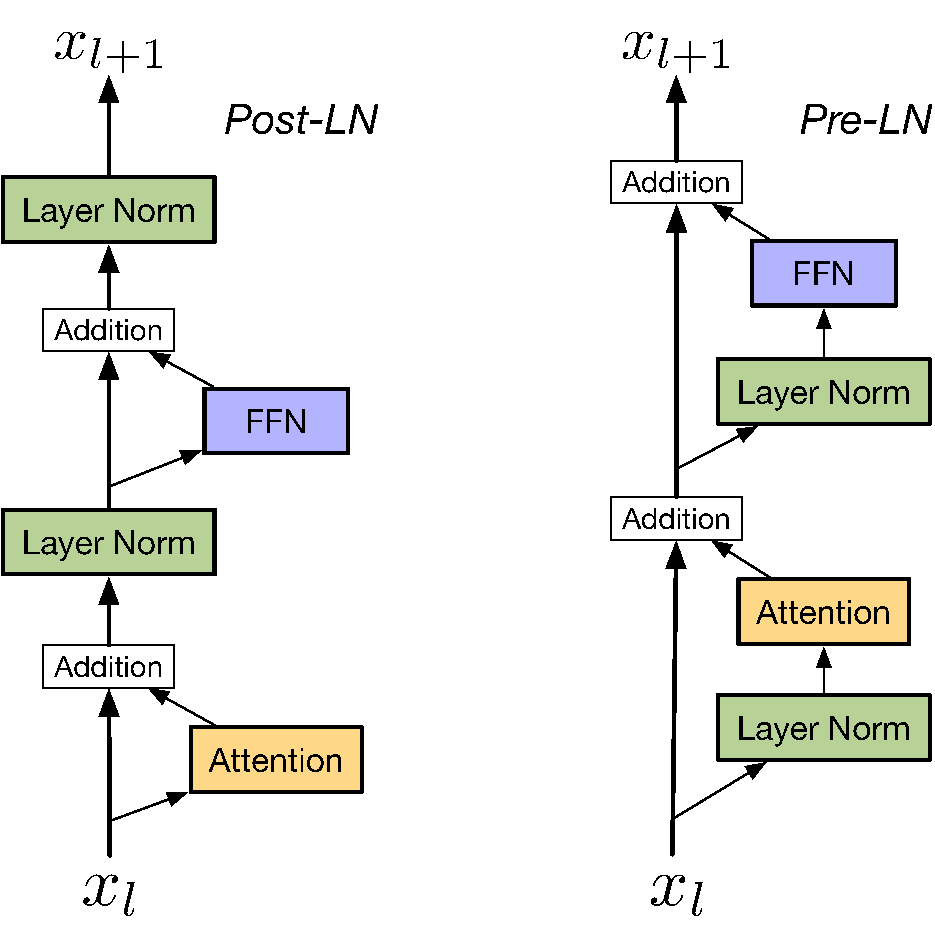
\includegraphics[width=0.7\textwidth]{figures/post-vs-pre-norm.pdf}
    \caption{Comparison of post-normalization and pre-normalization architectures in Transformer models}\label{fig:post-vs-pre-norm}
    \hfill\textit{Source: \citet{ding2021}}
\end{figure}

\subsection{Normalization}

The normalization layer stabilizes the training process by normalizing the input embeddings independently for each token. Various types of normalization layers exist. While the original architecture used layer normalization \parencite{ba2016}, root mean square layer normalization \parencite{zhang2019} has also been widely adopted.

\subsection{Attention}

Consider two additional architectural parameters \(d_k\) and \(d_v = d_{\mathrm{model}}\). The attention layer is described using three weight matrices: \(\mathbf{W}_Q, \mathbf{W}_K \in \mathbb{R}^{d_k \times d_{\mathrm{model}}}\) and \(\mathbf{W}_V \in \mathbb{R}^{d_v \times d_{\mathrm{model}}}\). The output of the layer is calculated as follows:
\begin{equation}\label{eq:attention}
    \mathrm{Attention}(\mathbf{Q}, \mathbf{K}, \mathbf{V}) = \mathrm{softmax}\left(\frac{\left[\mathbf{QK}^\top\right]_{\mathrm{mask}}}{\sqrt{d_k}}\right)\mathbf{V},
\end{equation}
where \(\mathbf{V} = \mathbf{XW}_V^{\top}\) and \(\{\mathbf{Q}, \mathbf{K}\} = \mathrm{RoPE}(\mathbf{XW}_{\{Q, K\}}^\top)\) with \(\mathrm{RoPE}\) denoting the rotary position embedding discussed in \sectionref{sec:rotary-position-embedding}. The softmax is applied row-wise, and \([\ \cdot \ ]_{\mathrm{mask}}\) is a causal masking operation that sets all elements above the main diagonal to \(-\infty\), thereby preventing data leakage from future tokens.

\begin{figure}[ht]
    \centering
    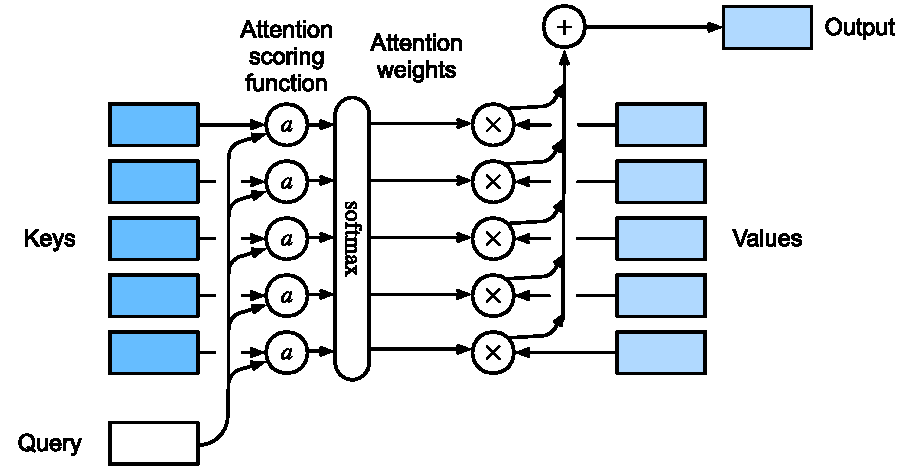
\includegraphics[width=0.85\textwidth]{figures/attention.pdf}
    \caption{Attention mechanism at the single token level}\label{fig:attention}
    \hfill\textit{Source: \citet{zhang2023b}}
\end{figure}

Attention functions as a layer that enables tokens to communicate with each other. Each token performs a query \(\mathbf{q}_i\) to all preceding tokens and itself \(\mathbf{k}_{j \le i}\). The corresponding attention weight of the query-key match \(\mathbf{q}_{i}^\top\mathbf{k}_{j}\) is normalized by the softmax and used as a soft dictionary lookup to retrieve the partial component of the value vector \(\mathbf{v}_j\). The convex combination of all such value vectors \(\mathbf{v}_{j \le i}\) becomes the output of the attention layer. This operational flow for a single query is illustrated in \figureref{fig:attention}.

\subsection{Multi-Head Attention}

Multi-head attention is a modification of the basic attention mechanism. Instead of applying the attention mechanism once, the embedding processing is divided into multiple heads that perform attention in parallel. Given the number of heads \(h\) and an additional output projection weight matrix \(\mathbf{W}_O \in \mathbb{R}^{hd_v \times d_{\mathrm{model}}}\), the output of the layer is calculated as:
\begin{align}
    \mathrm{MultiHead}(\mathbf{X}) &= \\ \mathrm{MultiHead}(\mathbf{Q}, \mathbf{K}, \mathbf{V}) &= \mathrm{Concat}(\mathrm{head}_1, \ldots, \mathrm{head}_h) \mathbf{W}_O \\
    \text{where}~\mathrm{head_i} &= \mathrm{Attention}(\mathbf{Q}_i, \mathbf{K}_i, \mathbf{V}_i),
\end{align}
where \(\mathbf{Q}_i, \mathbf{K}_i, \mathbf{V}_i\) are obtained by applying an independent set of weight matrices \(\mathbf{W}_Q^{(i)}, \mathbf{W}_K^{(i)}, \mathbf{W}_V^{(i)}\) to the input embeddings \(\mathbf{X}\), and \(\mathbf{Q}, \mathbf{K}, \mathbf{V}\) are their concatenated versions.

In this version of the attention, \(d_v\) is not necessarily equal to \(d_{\mathrm{model}}\).

\subsection{Multi-Layer Perceptron}

A multi-layer perceptron (MLP) is a simple feed-forward neural network with two linear transformations and a non-linear activation function. It is applied to each token independently.

Originally, the rectified linear unit (ReLU) was used as the activation function. However, other alternatives have empirically been shown to perform better. Two of these are the Gaussian error linear unit (GELU) and the sigmoid linear unit (SiLU) from \citet{hendrycks2016}. Another is the swish gated linear unit (SwiGLU) introduced in \citet{shazeer2020}.

\subsection{Dropout}

Dropout is a widely adopted regularization technique that enhances the generalization of the model \parencite{srivastava2014}. During the training process, it randomly masks some of the activations of the preceding layer with a probability \(p_{\mathrm{dropout}}\) and scales the remaining activations by a factor of \(1 / p_{\mathrm{dropout}}\) to maintain the output statistics of the layer. This process is conceptually illustrated in~\figureref{fig:dropout}.

\begin{figure}[ht]
    \centering
    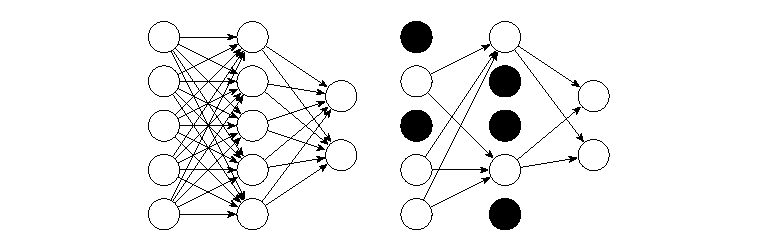
\includegraphics[width=\textwidth]{figures/dropout.pdf}
    \caption{An application of dropout to a multi-layer perceptron}\label{fig:dropout}
    \hfill\textit{Source: \citet{labach2019}}
\end{figure}

This method is frequently applied in transformers across all layers, including the dropout of the attention scores calculated before the application of the softmax function. (\cite{vaswani2017};~\cite{zehui2019})

\subsection{Rotary Position Embedding}\label{sec:rotary-position-embedding}

Rotary Position Embedding (RoPE) is a modification built upon the vanilla Transformer to incorporate the positional information of tokens and address issues present in the originally proposed analogous approach. RoPE was introduced by \citet{su2021} and quickly gained widespread adoption.

For each embedding \(\mathbf{x}_m\) at position \(m\) in the sequence, RoPE proposes a rotation of its query and key vectors:
\begin{equation}
	\{\mathbf{q}_m, \mathbf{k}_m\} = \mathrm{RoPE}(\mathbf{W}_{\{Q, K\}}\mathbf{x}_m, m) = \mathbf{R}^d_{\Theta, m}\mathbf{W}_{\{Q, K\}}\mathbf{x}_m 
\end{equation}
using an orthogonal rotary matrix  
\begin{equation}    
	\mathbf{R}^d_{\Theta,m} = 
	\scalebox{0.8}{\(
	\begin{pmatrix}
		\cos{m\theta_1}& -\sin{m\theta_1}&0&0&\cdots&0&0\\
		\sin{m\theta_1}&\cos{m\theta_1}&0&0&\cdots&0&0 \\
		0&0&\cos{m\theta_2}& -\sin{m\theta_2}&\cdots&0&0\\
		0&0&\sin{m\theta_2}&\cos{m\theta_2}&\cdots&0&0 \\
		\vdots&\vdots&\vdots&\vdots&\ddots&\vdots&\vdots\\
		0&0&0&0&\cdots&\cos{m\theta_{d/2}}& -\sin{m\theta_{d/2}}\\
		0&0&0&0&\cdots&\sin{m\theta_{d/2}}&\cos{m\theta_{d/2}}
	\end{pmatrix}
	\)},
\end{equation}
where \(d = d_k\) and \(\Theta = \{\theta_i=\theta_{\mathrm{base}}^{-2(i-1)/d}, i \in \{1, 2, \ldots, d/2\}\}\) is a predefined set of frequencies derived from the base frequency hyperparameter \(\theta_{\mathrm{base}}\). RoPE can be interpreted as a rotation of two-dimensional scalar chunks of the query and key vectors, determined by both the token's position within the sequence and the chunk's position within the vector, as illustrated in \figureref{fig:rope}.

\begin{figure}[ht]
    \centering
    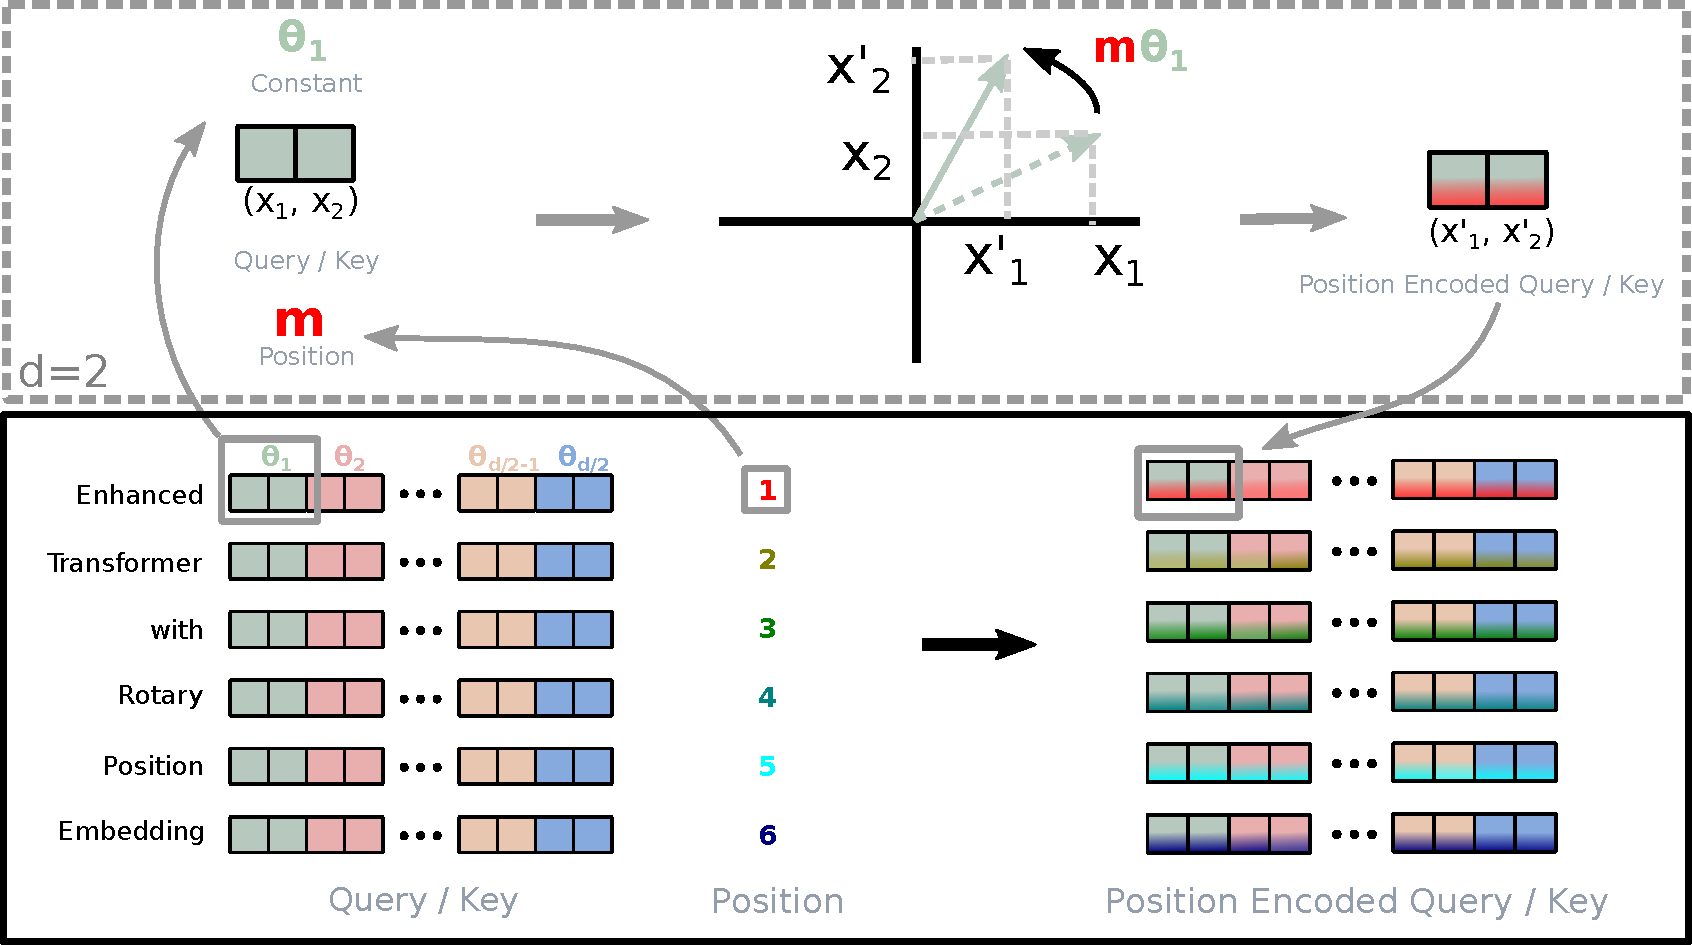
\includegraphics[width=\textwidth]{figures/rope.pdf}
    \caption{Illustration of the effect of RoPE on the query and key vectors}\label{fig:rope}
    \hfill\textit{Source: \citet{su2021}}
\end{figure}

Note two important details regarding the application of RoPE. First, it requires \(d\) to be even. Second, it is applied across all heads in multi-head attention without repeating the rotation frequency \(h\) times, inherently adding more functional bias to heads working on higher frequencies \parencite{barbero2024}.

When multiplying query and key matrices in \equationref{eq:attention}, the two embeddings \(\mathbf{x}_m\) and \(\mathbf{x}_n\) derive the attention score decay based on the relative distance \(m-n\) between them:
\begin{equation}
	\mathbf{q}_m^{\top}\mathbf{k}_n
	=(\mathbf{R}^d_{\Theta, m}\mathbf{W}_Q\mathbf{x}_m)^\top(\mathbf{R}^d_{\Theta, n}\mathbf{W}_K\mathbf{x}_n) =\mathbf{x}_m^\top\mathbf{W}_Q\mathbf{R}^d_{\Theta, n-m}\mathbf{W}_K\mathbf{x}_n,
\end{equation}
which allows the model to capture the positional information of the tokens.

\section{Training}

To elaborate on the process of convergence from a randomly initialized model to one with desirable properties, this section provides an overview of the training process by deriving the direct objective and describing the optimization algorithm, along with associated batch-related terminology and learning rate scheduling.

\subsection{Maximum Likelihood Estimation}

Training the language model \(p_\theta\) involves aligning the distribution it represents with the true data distribution. However, the later is unknown, and only a finite set \(\mathcal{D} = \{\bm{x}^{(1)}, \bm{x}^{(2)}, \ldots, \bm{x}^{(n)}\}\) of instances sampled from it is available. The training objective \(\mathcal{L}_{\mathcal{D}}\), known as the likelihood function, is expressed as the probability of these samples being generated by the model. Assuming that samples are independent and identically distributed, \(\mathcal{L}_{\mathcal{D}}\) can be decomposed into the product of individual probabilities:
\begin{equation}
	\mathcal{L}_{\mathcal{D}}(\theta) = p_{\theta}(\bm{x}^{(1)}, \bm{x}^{(2)}, \ldots, \bm{x}^{(n)}) = \prod_{i=1}^{n} p_{\theta}(\bm{x}^{(i)}) \rightarrow \max.
\end{equation}
The method of estimating the parameters \(\theta\) by maximizing this function is called maximum likelihood estimation (MLE).

Due to several reasons, including underflow issues, the log-likelihood function is often used instead:
\begin{equation}
	\ell_{\mathcal{D}}(\theta) = \log \mathcal{L}_{\mathcal{D}}(\theta) = \log \prod_{i=1}^{n} p_{\theta}(\bm{x}^{(i)}) = \sum_{i=1}^{n} \log p_{\theta}(\bm{x}^{(i)}).
\end{equation}
Optimizing both functions is equivalent, as the logarithm is a monotonically increasing function.

To take one step further, a minus sign can be added to focus on minimization instead of maximization, thereby formulating the negative log-likelihood loss function. Additionally, \equationref{eq:probability-chain-rule} can be used to express the loss function as a sum of the log-likelihoods of the individual tokens:
\begin{equation}
	L(\theta) = -\ell_{\mathcal{D}}(\theta) = -\sum_{i=1}^{n} \sum_{t=1}^{T_i} \log p_{\theta}(x^{(i)}_t \mid \bm{x}^{(i)}_{1:t-1}) \rightarrow \min.
\end{equation}
This objective corresponds to the cross-entropy (CE) loss, which is often represented using the dot product of \(\mathbf{p}^{(i)}_t\) from \equationref{eq:softmax} and the one-hot encoding of the target token \(x^{(i)}_t\).

\subsection{Gradient-Based Optimization}

Various optimization algorithms have been developed to train neural networks. The most effective ones are based on first-order methods, which iteratively adjust the parameters by subtracting the stochastic gradient of the loss function with respect to the parameters. The degree of this adjustment is controlled by multiplicative factor of the gradients called learning rate. Gradients are calculated using a subsample of the training set, known as a mini-batch (or simply batch), with the application of automatic differentiation.

In the field of language modeling, the adaptive moment estimation (Adam) \parencite{kingma2014}, a modification of stochastic gradient descent (SGD), and its version supporting weight decay \parencite{loshchilov2017} are the most popular algorithms. Adam maintains two moving average statistics, called the first and second moments, for each parameter, which correct the application of the gradient and accelerate convergence.

Training is sometimes conducted using a half-precision floating-point format to increase computational speed. However, this approach introduces the risk of underflow for small gradient values. To mitigate this issue, \textit{gradient scaling} is employed. This technique multiplies the loss value by a constant factor, allowing the gradients to maintain appropriate magnitudes during backpropagation. When the optimization step is performed, the gradients are rescaled by the same factor to restore the original learning rate setting. The scaling factor is often determined automatically. \parencite{nvidia2024}

\begin{sloppypar}
Another common modification applied to gradients is \textit{clipping}, which projects the gradient vector onto the surface of a hypersphere with a radius equal to a predefined value if its norm exceeds this threshold. This process prevents gradients from exploding in regions with sharp loss landscapes and stabilizes the training process. \parencite{pascanu2013}
\end{sloppypar}

\subsection{Batch-Related Terminology}

Due to the operational nature of graphics processing units (GPUs), multiple sequences must be organized to have the same length to be processed in parallel. This is achieved by either padding shorter sequences with special tokens or truncating longer ones. The model's scope of visibility is termed the context window, and its size is referred to as the context length.

In some cases, sequences are randomly shuffled, concatenated, and split to form batches without the need for padding or truncation. This technique is known as batch packing.

When hardware constraints limit batch size, gradient accumulation is utilized. Instead of using the entire batch for a single optimization step, it is divided into micro-batches, which are processed sequentially. The parameters are updated only after all the micro-batches have been processed.

\subsection{Learning Rate Scheduling}

Due to the design of Adam, a few iterations at the beginning of training are required to gather sufficient gradient statistics for better moment estimation. This requirement becomes even more critical in the context of the instability associated with Transformers. During this initial phase, using the full learning rate is inadvisable, as it may lead to unstable updates. To mitigate this issue while utilizing all available data, a warm-up period is introduced in the training process. Throughout this period, the learning rate is gradually increased, often linearly, from zero to the desired value over a predefined number of iterations.

After training with high learning rates, the model benefits from smaller parameter updates as it approaches the local optimum and requires more precise adjustments. This is achieved by decaying the learning rate over time.

To summarize, the learning rate, rather than being a constant hyperparameter, has evolved into a function of the iteration index, thereby opening a new dimension for controlling the training process.

\section{Inference}\label{sec:inference}

This section introduces the fundamental concepts related to the inference process of language models, specifically sampling and stopping criteria.

\subsection{Sampling}\label{sec:sampling}

As previously mentioned, a language model represents a probability distribution over the vocabulary given the preceding context. The iterative process of sampling from this distribution and incorporating these new tokens into the model's context is referred to as generation.

Tokens are selected based on their associated probabilities \(\mathbf{p}_t\) from the softmax output, as described in \equationref{eq:softmax}. The temperature parameter modulates the sharpness of this distribution. There are two limiting cases, which are demonstrated in \figureref{fig:softmax-temperature}: First, as \(\tau \to +\infty\), the distribution becomes uniform, with all tokens having an equal probability of being selected. Second, as \(\tau \to 0^+\), the selection becomes deterministic, choosing the most probable token. This is known as greedy decoding and corresponds to the greedy search algorithm in a graph of all possible sequences, where the language model functions as a heuristic.

\begin{figure}[ht]
    \centering
    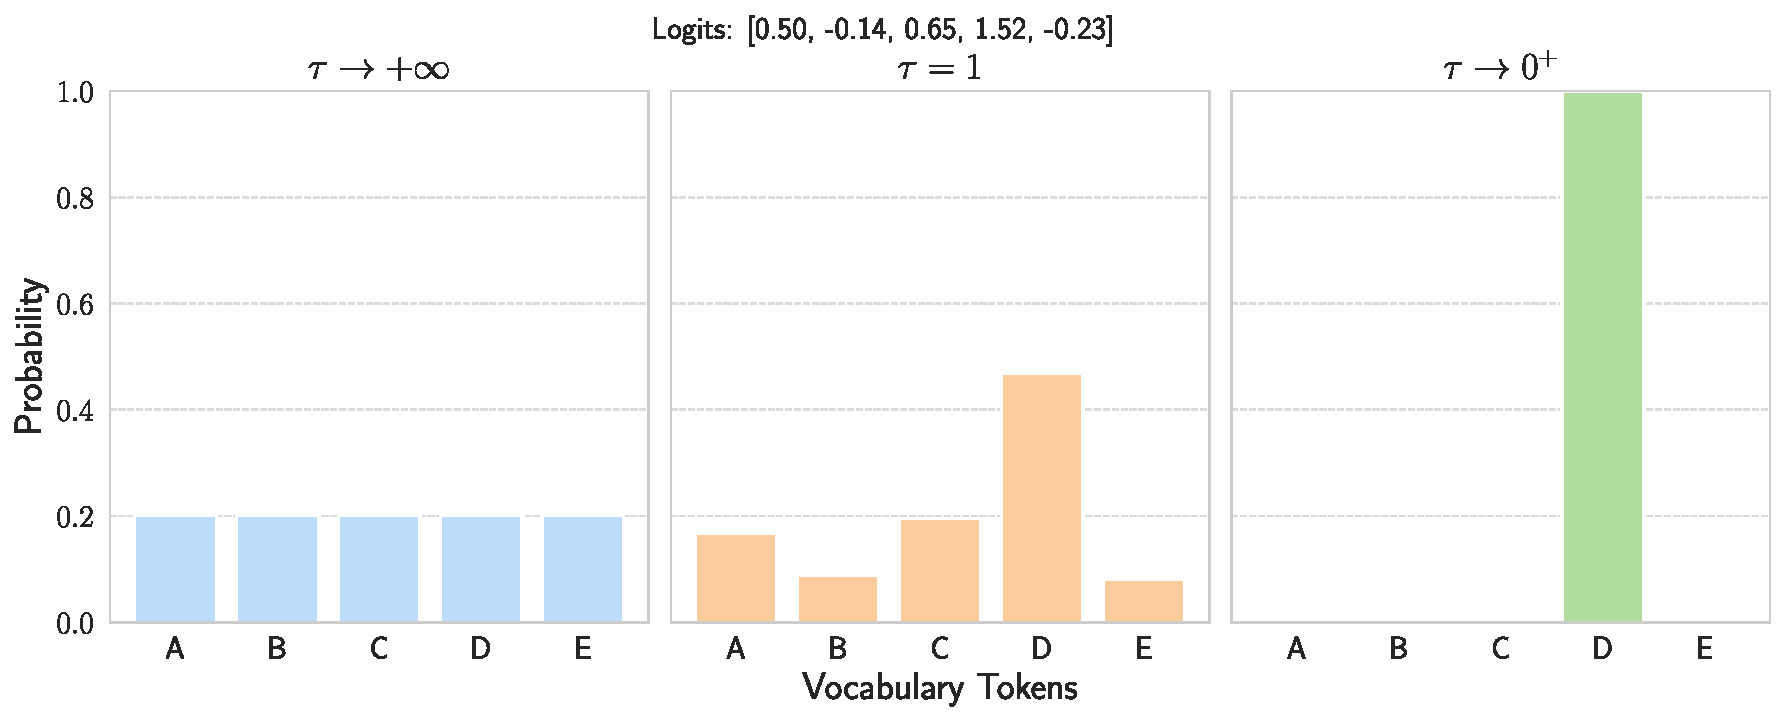
\includegraphics[width=\textwidth]{figures/softmax-temperature.pdf}
    \caption{Impact of the temperature parameter on the softmax output}\label{fig:softmax-temperature}
\end{figure}

To further enhance the quality of the generated text, the top-\(k\) sampling strategy is often employed. It restricts the vocabulary to the top-\(k\) most probable tokens, which helps prevent the model from outputting irrelevant tokens.

A similar concept is applied in the nucleus sampling strategy, also known as top-\(p\) sampling \parencite{holtzman2019}. It restricts the vocabulary to the smallest set of tokens whose cumulative probability exceeds a threshold parameter \(p\).

\subsection{Stopping Criteria}

There are several methods to terminate the generation process.

Firstly, the model can signal the completion of the output sequence by generating an end of sequence (EOS) token. This requires the EOS token to be included in the vocabulary, and the model must be trained to produce it. This is accomplished by appending the EOS token to the end training sequences.

Secondly, algorithmic stopping criteria can be employed. For example, the generation process can be halted when a maximum length threshold is exceeded. Another pertinent example, particularly in the context of code completion, is to cease generation when the model outputs a token containing a newline character.

\chapter{Completion-Centric LM}

% TODO: description

\section{Training Stages}

The training of modern Code LLMs begins with acquiring a model checkpoint that possesses a robust understanding of code. This can be achieved through two distinct types of training stages. One type involves taking a general-purpose pre-trained LLM and fine-tuning it on a file-level code dataset. This approach is utilized by models such as Code Llama \parencite{rozière2023} and Qwen2.5-Coder \parencite{hui2024}. The other type involves training a model from scratch using a mixture of code and code-related natural language data. This pre-training approach is adopted by models like DeepSeek-Coder \parencite{guo2024} and OpenCoder \parencite{huang2024}. Both types necessitate vast amounts of data, typically ranging from 2 trillion (2T) to 18 trillion (18T) tokens with context length of 4,096 (4K). 

Once a strong model with a limited context size is trained, it often undergoes repository-level pre-training (sometimes referred to as long-context fine-tuning). The objective of this stage is to extend the context window, thereby enabling the model to comprehend a broader scope within a given repository. Unlike the initial training stage, repository-level pre-training requires significantly fewer tokens. However, it necessitates the application of context extrapolation methods and the utilization of longer input sequences. This phase typically involves between 8 billion (8B) and 300 billion (300B) training tokens, with the context window extended with 16K or 32K tokens.

% TODO: forward reference to the tiny paper results

Each input sequence in repository-level pre-training consists of two components: the composed context and the completion file. Various methods exist for obtaining the former. In this thesis, the function responsible for this task is referred to as the context composer, or simply composer. This process involves retrieving and preprocessing a subset of files, which are then assembled to form a repository context.

Models trained using only the aforementioned stages are referred to as base models. To enhance their utility for various tasks, an additional instruction tuning phase is often conducted. However, the capabilities gained from this stage are not essential for the code completion task and are not discussed further in this thesis. Throughout this work, all mentioned models are assumed to be their base versions.

\section{Gradient Masking}

The learning signal for the model is derived from both the composed context and the completion file sources. The alignment of their distributions is contingent upon the specific choice of the composer. When learning the completion of all tokens, a mismatch in these distributions can introduce undesirable bias into the model.

For instance, learning to complete README files may be irrelevant if the model's primary objective is to excel solely in code completion. However, incorporating various file formats into the context is justified if they hold relevance to the completion task (e.g., including documentation).

This issue can be mitigated through the application of gradient masking. By setting the individual losses of non-completion tokens to zero, these tokens can be excluded from the gradient computation during training.

% TODO: forward reference to the practical discussion on this subject

\section{Fill-in-the-Middle}\label{sec:fill-in-the-middle}

Due to the autoregressive nature of decoder-only Transformers, they are unable to utilize future tokens in their context. Consequently, to account for both the prefix and suffix of the completion file, the fill-in-the-middle approach was proposed by \citet{bavarian2022}, with its origins in the works of \citet{donahue2020}, \citet{aghajanyan2022}, and \citet{fried2022}. This capability is particularly advantageous for the completion task, as code is frequently written in a non-sequential and chaotic order.

The primary concept of FIM involves randomly dividing a portion of training sequences into three segments: prefix, middle, and suffix. These segments are then concatenated using special tokens to form a new sequence order: prefix, suffix, and middle. Incorporating such augmented data into the pre-training process, introduces a new capability to the model, albeit with a marginal performance degradation (\cite{allal2023};~\cite{rozière2023}).

% TODO: BPE-dropout, starting generation from the middle of the token?

\section{Evaluation}

% TODO: metric x benchmark table?
% TODO: modes of evaluation: teacher forcing

\subsection{Metrics}

% TODO: Keep in mind: effect of the number of preceding tokens -> not a uniform measure across the context

\subsubsection*{Exact Match}

The exact match (EM) metric is a fundamental and widely used measure for evaluating code completion. It is defined as the ratio of correctly completed code lines to the total number of lines. This metric is particularly valued for its direct alignment with the objectives of code completion evaluation.

However, the exact match metric operates at a line-level granularity, which means it only indicates whether a line is completed correctly or not. This binary nature of the metric does not offer insights into the degree of deviation from the correct completion in cases where the completion is incorrect. To mitigate this limitation, the exact match metric is often used in conjunction with the more granular measures.

\subsubsection*{Edit Similarity}

The generation of functionally correct code completions is valuable, yet the effort required to edit and adapt these generated lines is equally significant. Edit similarity (ES) quantifies this effort by measuring the number of single-character edits (insertions, deletions, or substitutions) needed to transform the generated code into a reference \parencite{svyatkovskiy2020}. Mathematically, ES for two strings is expressed as:
\begin{equation}
    \text{\textsc{ES}}(\bm{x}, \bm{y}) = 1 - \frac{\mathrm{lev}(\bm{x}, \bm{y})}{\max\{|\bm{x}|, |\bm{y}|\}},
\end{equation}
where \(\mathrm{lev}(\bm{x}, \bm{y})\) represents the Levenshtein distance between the generated code \(\bm{x}\) and the reference sample \(\bm{y}\), and \(|\cdot|\) denotes the length of the string.

This metric is crucial for evaluating code completion scenarios, as it provides a measure of the effort developers must exert to correct errors in the generated code. Moreover, it has been shown that edit similarity moderately correlates with the generation of functionally correct code \parencite{dibia2022}.

\subsubsection*{Cross-Entropy \& Perplexity}

As mentioned earlier, cross-entropy is employed as a loss function in the training process of language models. More specifically, it represents the average log-likelihood of the individual ground truth tokens. It can also be interpreted as the average number of nats required to encode the model's predictions per token compared to the true distribution.

Perplexity (PPL) is the exponentiated form of cross-entropy, providing a more intuitive interpretation as the average number of choices among which the model is uncertain. For this reason, perplexity is often referred to as the weighted average branching factor of a language \parencite{murphy2022}.

Both metrics are frequently used as proxies for assessing model quality. They are valuable for monitoring because these measures are consistently computed during training, being either derived from the loss function (PPL) or representing the loss itself (CE). However, they are too abstract to serve as primary metrics for specific tasks. Additionally, these measures are heavily influenced by vocabulary size and tokenization methods, which makes them unsuitable for comparing different models.

\subsubsection*{Top-\(k\) Accuracy}

Top-\(k\) accuracy is a metric that quantifies the frequency with which the model's top-\(k\) predictions align with the actual ground truth completion. Within the scope of this thesis, top-\(k\) accuracy is considered as a token-level metric to provide a more granular evaluation of the model's performance.

\subsubsection*{Pass@k}

\begin{sloppypar}
All aforementioned metrics are syntax-based, meaning they evaluate the model's performance based on the syntactic match between the generated and reference completions. However, in real-world scenarios, there exists a wide variety of correct completions that may not be present in the dataset used for evaluation. The model might predict a completion that fulfills the user's functional requirements, even if the metric evaluates it as incorrect.
\end{sloppypar}

To address this issue, an unbiased estimation of the probability that at least one generated solution out of \(k\) passes all unit tests was proposed by \citet{chen2021}. This metric, known as pass@k, is calculated using the following expectation:
\begin{equation}
    \text{pass@k} = \underset{\mathrm{Problems}}{\mathbb{E}}\left[1 - \frac{\binom{n-c}{k}}{\binom{n}{k}}\right],
\end{equation}
where \(n \ge k\) is the number of samples generated by the model, and \(c \le n\) is the number of those samples that passed all unit tests. This metric reflects the probability of finding a correct solution within \(k\) attempts, which mirrors the iterative approach developers often take when exploring multiple solutions.

To apply this metric to single-line code completion, it is assumed that all other lines, except the target one, are present and functionally correct. This assumption does not hold for many use cases, such as when a user writes a function on the fly. Therefore, pass@k offers an optimistic assessment of completion capabilities, as the evaluation set contains one corrupted line per problem. This metric is more realistic for tasks with greater completion granularity or for code generation tasks.

% TODO: in practical part: motivate why this metric is not used 

\subsubsection*{Other Metrics}  % TODO: better name

% TODO: BLEU
% TODO: BLEU4
% TODO: CodeBLEU
% TODO: ChrF
% TODO: ROUGE, ROUGE-N, ROUGE-L, ...
% TODO: METEOR
% TODO: BERTScore
% TODO: Ruby
% TODO: Jaccard Similarity



\subsection{Evaluation Modes}

\subsection{Benchmarks}

% TODO: RepoBench
% TODO: Long Code Completion: https://arxiv.org/abs/2306.14893
% TODO: LCA
% TODO: Codev-Bench
% TODO: CrossCodeEval
% TODO: CrossCodeLongEval
% TODO: RepoEval
% TODO: RepoMasterEval
% TODO: EvoCodeBench
% TODO: CoderEval
% TODO: CodeXGLUE
% TODO: BigCodeBench
% TODO: R2C2-Bench
% TODO: M2RC-EVAL

\chapter{In-Context Learning}\label{chap:in-context-learning}

There will be:
\begin{itemize}
    \item Definition of in-context learning (ICL),
    \item References to studies supporting the usefulness of ICL for repository-level code completion capabilities of Code LLMs,
    \item Discussion on prompt engineering,
    \item Comparison of zero-shot, one-shot, and few-shot learning.
\end{itemize}


\makeatletter
\def\@part[#1]#2{%
  \ifnum \c@secnumdepth >-2\relax
    \refstepcounter{part}%
    \renewcommand{\@currentlabelname}{#1}%
    \addcontentsline{toc}{part}{\thepart\hspace{1em}#1}
  \else
    \addcontentsline{toc}{part}{#1}
  \fi
  \markboth{}{}%
  {\centering
    \interlinepenalty \@M
    \normalfont
    \ifnum \c@secnumdepth >-2\relax
      \huge\bfseries \partname\nobreakspace\thepart
      \par
      \vskip 20\p@
    \fi
    \Huge \bfseries #2\par
    \vskip 0.5cm
    \normalsize\normalfont\textit{The investigation of the final research question, \hyperref[rq:rq-b2]{RQ.B2}, in this thesis was previously published by \citet{sapronov2025} in the ``Tiny Papers'' track at the Deep Learning for Code (DL4C) workshop during the International Conference on Learning Representations (ICLR) 2025. This thesis should be regarded as an extended version of that paper, authored by the same individual, and does not constitute plagiarism of either their own or others' work. All differences are highlighted and justified below.}\par}
  \@endpart}
\makeatother

\part{Applied Research}\label{part:applied-research} % other options are Experimental Analysis, Research Part, Experimental Validation
\addtocontents{toc}{\protect\vspace{-\baselineskip}}
% TODO: tiny paper disclaimer

\chapter{Technical Foundation}\label{chap:technical-foundation}  % other option are Framework Design, Implementation Details

This chapter offers a comprehensive description of the context composition framework and the fine-tuning pipeline employed in the research presented in this thesis. Additionally, it includes a list of tools necessary for executing their implementations.

\section{Context Composition Framework}

This section begins with an explanation of the independent building blocks of the context composition framework and their integration to form a complete compositional strategy. It then enumerates all the composers utilized in the experimental section, accompanied by their descriptions. Finally, it offers an overview of the additional parameter applied to modify the retrieval order and includes a commentary that invites further exploratory investigation into the framework.

\subsection{Building Blocks}

As stated in Section~\ref{sec:training-stages}, we define the context composer as a function that takes a repository snapshot and a completion file and returns a string that represents the project context. This function is decomposed into seven abstract blocks:

\begin{enumerate}
    \item \textbf{File Filtering} determines which files to include in the subsequent data processing pipeline. For instance, it can filter out files with empty content or files with certain extensions.
    \item \textbf{File Preprocessing} modifies the content of the files. For example, it can extract code from markdown files.
    \item \textbf{File Chunking} changes the granularity of the data from files to text chunks. The simplest form of chunking is identity, which maintains the file-grained structure.
    \item \textbf{Chunk Ranking} determines the relevance of the chunks for the completion file. It can take multiple forms, ranging from simple heuristics and sparse embedding comparisons to more sophisticated dense approaches.
    \item \textbf{Chunk Sorting} defines the rules for ordering the chunks based on their ranks. The most common scenario is to sort the chunks in ascending order of their ranks, placing the most relevant chunks at the end of the list.
    \item \textbf{Chunk Assembling} joins sorted chunks into a single string using a specific template. For example, the assembler can prepend a comment with path information of the chunk's source file and join them using a separator string.
    \item \textbf{Context Postprocessing} modifies the context as a unified string. For instance, line dropout can be applied by this block.
\end{enumerate}

Each of these blocks has its own abstract class and serves as a foundation for concrete implementations. This design allows for several different transformations associated with a single block type to be part of a single context composer, eliminates code duplication and allows for greater flexibility in composer creation. The directed graph presented in Figure~\ref{fig:composer-blocks} visualizes the order in which these instances can be applied.

\begin{figure}[ht]
    \centering
    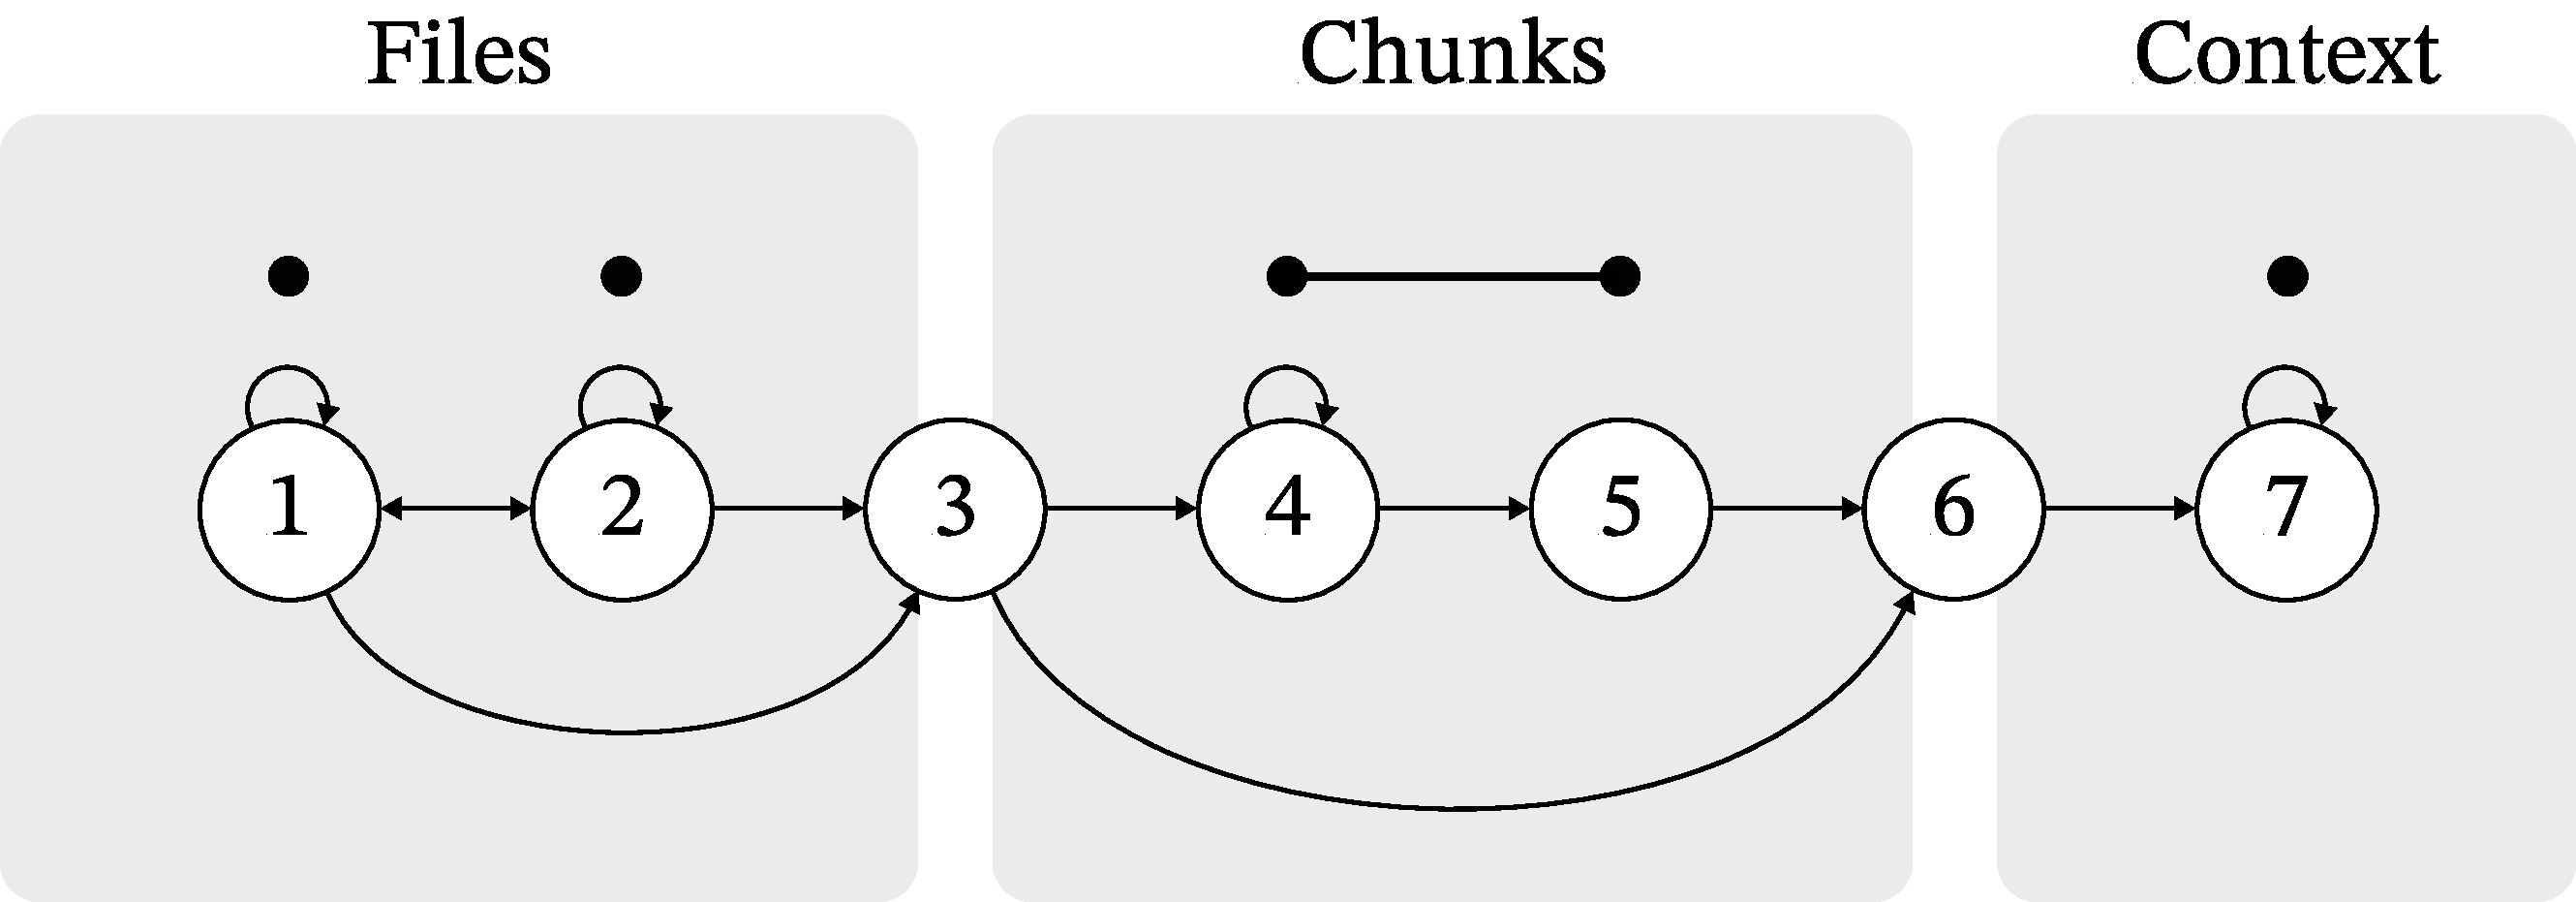
\includegraphics[width=\textwidth]{figures/composer-blocks.pdf}
    \caption{Order of composer blocks. Nodes represent block types: \textcircled{\raisebox{-0.9pt}{1}} File Filtering, \textcircled{\raisebox{-0.9pt}{2}} File Preprocessing, \textcircled{\raisebox{-0.9pt}{3}} File Chunking, \textcircled{\raisebox{-0.9pt}{4}} Chunk Ranking, \textcircled{\raisebox{-0.9pt}{5}} Chunk Sorting, \textcircled{\raisebox{-0.9pt}{6}} Chunk Assembling, and \textcircled{\raisebox{-0.9pt}{7}} Context Postprocessing. Edges indicate the permissible sequence of block application. The data format is denoted by three frames: Files, Chunks, and Context. The bold subgraph highlights blocks that may be omitted.}\label{fig:composer-blocks}
\end{figure}

\subsection{List of Context Composers}

All context composers utilized in the \nameref{chap:research-investigation} chapter adhere to two standard preprocessing steps: the removal of empty files and the normalization of all line endings to the Line Feed (LF) character. These shared preprocessing steps ensure consistency across all experiments. The following list provides a comprehensive overview of the context composers employed in this research.

\label{appendix:context-composers}
\begin{enumerate}
    \item \textbf{File-Level} produces an empty context.
    \item \textbf{Path Distance \texttt{.py}} constructs the context using only files with the \texttt{.py} extension. The selected files are sorted in descending order according to their path distance from the completion file. For files with identical path distances, a secondary sorting criterion is applied using the Intersection over Union (IoU) metric, which equals to the number of lines shared with the completion file divided by the total number of unique lines in both files. The IoU calculation considers lines with leading and trailing whitespace removed and includes only those lines that are at least five characters in length after whitespace removal.
    \item \textbf{Lines IoU \texttt{.py}} is similar to the Path Distance \texttt{.py} method, but omits the initial sorting by path distance. Instead, files are ranked directly using the IoU metric.
    \item \textbf{Code Chunks} removes all docstrings, comments, and import statements from the context produced by Path Distance \texttt{.py}.
    \item \textbf{Half-Memory \texttt{.py}} begins with the context generated by Path Distance \texttt{.py}. Each line is independently removed with a dropout probability of \(0.5\), maintaining the overall saturation of the context window.
    \item \textbf{Declarations \texttt{.py}} extends Path Distance \texttt{.py} by filtering out all non-declarative elements, retaining only function and class declarations.
    \item \textbf{Text Chunks \texttt{.py}} uses Path Distance \texttt{.py} as the base composer, but removes all code from the context, leaving only docstrings and comments.
    \item \textbf{Text Files} constructs the context using files with the extensions \texttt{.json}, \texttt{.yaml}, \texttt{.yml}, \texttt{.sh}, \texttt{.md}, \texttt{.txt}, and \texttt{.rst}. The selected files are grouped in ascending order of relevance: [\texttt{.json}], [\texttt{.yaml}, \texttt{.yml}], [\texttt{.sh}], [\texttt{.md}, \texttt{.txt}, \texttt{.rst}]. Within each group, files are further sorted in descending order according to their path distance from the completion file.
    \item \textbf{Random Files} constructs the context by randomly ordering all files from the repository snapshot.
    \item \textbf{Random \texttt{.py}} selects only files with the \texttt{.py} extension and arranges them in a random order.
    \item \textbf{Random Tokens} constructs the context by sampling a sequence of non-special tokens at random, with each token selected independently and with equal probability.
    \item \textbf{Duplication} constructs the context by repeatedly concatenating the content of the completion file until the maximum context window size is reached.
    \item \textbf{Leak} begins with the context produced by Path Distance \texttt{.py}. The completion file is randomly divided into five segments at newline characters, which then disjointedly replace context lines at random positions, approximately preserving the original token count.
\end{enumerate}
% TODO: motivate choices

\subsection{Order Modifications}

To increase the diversity of experiments conducted to address \hyperref[rq:rq-b1]{RQ.B1} and \hyperref[rq:rq-b2]{RQ.B2}, two additional file ordering modifications are considered alongside the \textit{original} mode, as illustrated in Figure~\ref{fig:order-modes}:

\begin{itemize}
    \item \textit{reversed}: The retrieved files that fit within the model's context window are reordered in reverse. Consequently, the most relevant file appears at the beginning of the context window.
    \item \textit{irrelevant}: The order of retrieved files is reversed prior to the context length cut-off, resulting in a complete reversal of the context, with the most irrelevant files positioned at the end of the context string.
\end{itemize}

\begin{figure}[ht]
    \centering
    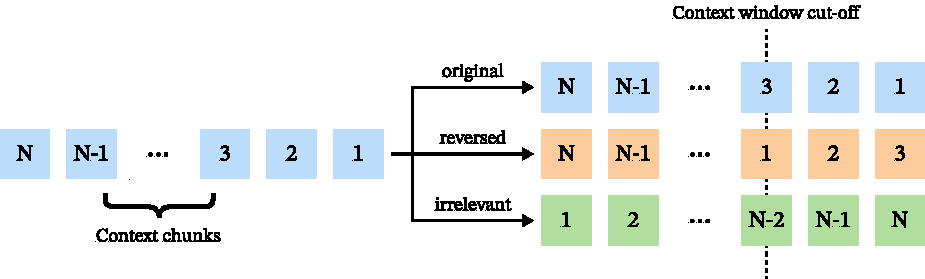
\includegraphics[width=\textwidth]{figures/order-modes.pdf}
    \caption{Three modes of context ordering. The numbers in boxes indicate the rank of the chunks, with smaller numbers denoting higher relevance.}\label{fig:order-modes}
\end{figure}

\subsection{Examples}

In addition to the blocks used to create composers employed in our experiments, we provide further exemplary implementations in the attached code, totaling 30 distinct blocks. The repository also includes a demonstrative Jupyter Notebook that describes these blocks and offers concrete usage examples of the package.

\section{Fine-Tuning Pipeline}

For the purposes of this research, we developed a fine-tuning pipeline aimed at adapting Code LLMs to the repository-level context.

From the data perspective, it supports the integration of pre-composed datasets obtained from the aforementioned context composition framework. The train-validation split is designed to eliminate data leakage from samples gathered from the same repositories. Configurable tokenization ensures context window saturation and facilitates the application of gradient masking.

The pipeline integrates models from the Hugging Face Hub\footnote{\url{https://huggingface.co/}}. It supports adapters that can augment the model architecture, freeze a subset of parameters, or modify the optimizer initialization. Models are dynamically loaded onto a single device based on hardware availability. Efficient attention implementation and parameter data types are selected using the same principle.

The training loop is implemented in pure PyTorch\footnote{\url{https://pytorch.org/}}. It supports cosine learning rate scheduling with linear warmup, gradient scaling, clipping, and accumulation. The pipeline can periodically invoke two validation loops: one on the original dataset split and another on an additional provided dataset. The latter allows metrics to be grounded on baseline composition strategy instead of solely monitoring the in-distribution capabilities of the model.

During the training process, the pipeline produces a set of configurable metrics and statistics for both the training and validation data. These include cross-entropy, exact match, top-\(k\) accuracy, learning rate tracking, epoch and token number counting. Their values are decomposed based on the types of tokens they are applied to. We denote five such types:
\begin{itemize}
    \item \textbf{Attached:} Tokens whose losses participate as leaf nodes in automatic differentiation for gradient computation.
    \item \textbf{Detached:} Tokens whose losses are zeroed out during gradient masking and serve as a complement to the attached tokens.
    \item \textbf{Completion:} Tokens of the completion file.
    \item \textbf{Context:} Tokens of the repository context.
    \item \textbf{Full:} All tokens.
\end{itemize}

In addition to statistics and metrics, the pipeline provides logging of the standard output and error streams. Checkpointing of the model and optimizer states is also supported.

The entire pipeline utilizes a modular structure, which enhances code maintainability and extendability. It is designed in an end-to-end manner, requiring only a pre-composed dataset, a set of YAML configuration files, and a single command line from the user. All components that employ stochastic behavior are accompanied by a seed parameter, ensuring that all experiments are reproducible.

\section{Tools}

In the context composition framework, we integrate Hugging Face tokenizers from the Transformers\footnote{\url{https://github.com/huggingface/transformers}} library to compute token-related statistics, and Tree-sitter\footnote{\url{https://tree-sitter.github.io/tree-sitter/}} to decompose Python code into its parts. Both libraries are employed in the concrete implementations of the blocks, although their usage can be omitted without disrupting the main abstract framework. The OmegaConf\footnote{\url{https://github.com/omry/omegaconf}} configuration system is utilized to manage the initialization of the composers from YAML configuration files.

The pipeline inherits requirements from the context composition framework as it utilizes its functions. Additionally, it employs Datasets\footnote{\url{https://github.com/huggingface/datasets}} and Accelerate\footnote{\url{https://github.com/huggingface/accelerate}} from the Hugging Face ecosystem to provide peripheral support to the Transformers library. The Hydra\footnote{\url{https://github.com/facebookresearch/hydra}} package extends the configurative capabilities of OmegaConf and enhances the pipeline's usability. PyTorch, as mentioned in the previous section, is used to implement the training loop. The tqdm\footnote{\url{https://github.com/tqdm/tqdm}} library is employed to display progress bars for all prolonged processes. Weights~\&~Biases\footnote{\url{https://github.com/wandb/wandb}} is used to track metrics and statistics in real-time.

To conduct all experiments and run evaluation scripts, a single 8\(\times\)H200 node was used, with each GPU having 141 GB of VRAM.

\chapter{Research Investigation}\label{chap:research-investigation}  % other option are Experimental Results, Research Exploration, Research Assessment

In this chapter we describe the research aspect of the thesis.  % TODO: add description 

\section{Research Questions}

To investigate the nature of in-context learning capabilities of Code LLMs, we consider the following research questions:

\begin{sloppypar}
\begin{description}
    \item[RQ.A1]\phantomsection\label{rq:rq-a1} \textbf{\nameref{sec:composition-impact-on-inference}:} Does the quality improvement of code completion depend on the composition strategy employed during model inference?
    \item[RQ.A2]\phantomsection\label{rq:rq-a2} \textbf{\nameref{sec:fine-tuning-on-compositions}:} Does fine-tuning a pre-trained Code LLM with a specific context composer enhance the subsequent quality of code completion?
    \item[RQ.B1]\phantomsection\label{rq:rq-b1} \textbf{\nameref{sec:effect-of-context-extension}:} Does the repository-level pre-training step affect the in-context learning abilities of the model developed during earlier stages?
    \item[RQ.B2]\phantomsection\label{rq:rq-b2} \textbf{\nameref{sec:influence-of-composition-on-context-extension}:} Does the quality improvement of code completion depend on the context composition approach used during the repository-level pre-training step?
\end{description}
\end{sloppypar}

\section{Experimental Design}

In this section, we describe the unified experimental design for all four research questions, including the data, training, and evaluation components. Specific details are deferred to the subsequent sections dedicated to each research question separately.

\subsection{Training Data}
% TODO: draw the diagram
% TODO: supporting company -> company that initialized this research
% TODO: mention JetBrains somewhere

The dataset utilized in this research was provided by the supporting company and is based on the methodology outlined in \citet{bogomolov2024}. The dataset was constructed by traversing the GitHub histories of Python repositories and applying permissive license filtering to sample completion files and their corresponding parent commits. Each data point consists of a pair: a list of Python completion files and a repository snapshot that captures the state of the repository at the time the completion files were added. The snapshot includes all text files except for the completion files themselves. To prevent contamination of the benchmark used in the evaluation, any repositories present in the benchmark were excluded from the training data.

To delineate the scope of this work, we ought to note that the corpus described thus far was entirely provided by the company and was not generated by the author of this thesis. Conversely, the subsequent processing steps applied to this dataset represent the original contributions of the author.

The multiple filtering criteria are applied to obtain the dataset with greater relevance and quality. First, all commits made prior to 2010 are excluded. Second, completion files with lengths outside the closed interval [800, 25000] characters are removed. Third, to eliminate redundancy, a simple deduplication strategy is employed on completion files based on the file name and the name of the repository to which they belong. Finally, up to 1000 of the most recently updated unique completion files are selected from each repository. The remaining repository snapshot is retained without additional processing. \parencite{sapronov2025}

The resulting corpus comprises 1,640 repositories, 160,801 commits, and 361,052 completion files. The completion files contain a total of 1.7 billion characters, while the repository snapshot files contain 4.8 trillion characters.

A subset of 2560 samples is randomly selected to form the validation set. During this process, we ensure that the repositories included in the training and validation sets do not overlap, and that no more than five different completion files are sourced from the same repository. After sampling for validation, the remaining data is sufficient to cover more than 250,000 unique completion files. We then apply the pre-composition procedure using the context composers listed in Section~\ref{sec:context-composers-list}. This allows us to perform this operation only once and reuse the smaller produced datasets for several experiments. Moreover, instead of saving the entire context string, which can reach the length of the total number of characters used in the repository, we apply a 16K-token cut-off, ensuring that the resulting datasets range from 4 to 17 GB in Parquet format. A demonstration of the first five data points of each dataset is provided in the accompanying thesis repository.

It is important to note that the pre-composition of both the training and validation sets is based on the entire completion file. This approach is motivated by the inefficiency of selecting target lines to possess file prefixes during the training and validation processes. For better clarity, one can consider training on a single line from each completion file; this results in the degradation of the gradient approximation proportional to the number of completion lines, or an increase in the number of forward and backward passes to the same degree.

\subsection{Training}

We utilize DeepSeek-Coder-Base 1.3B \parencite{guo2024} to address \hyperref[rq:rq-a1]{RQ.A1} and \hyperref[rq:rq-a2]{RQ.A2}, as it served as a robust foundation for code completion research at the inception of this work. It supports a context window size of 16K tokens, allowing us to leverage a substantial portion of the repository data. For experiments concerning \hyperref[rq:rq-b1]{RQ.B1} and \hyperref[rq:rq-b2]{RQ.B2}, we employ OpenCoder-1.5B-Base \parencite{huang2024}, the only modern Code LLM released without undergoing a repository-level pre-training stage. This model supports a maximum context window size of 4K tokens, providing an opportunity to explore context extension fine-tuning. For this purpose, we adjust the base frequency of RoPE from \(\theta_{\mathrm{base}} = 10{,}000\) to \(\theta_{\mathrm{base}} = 500{,}000\), as it was concurrently proposed by \citet{rozière2023} and \citet{xiong2023}. % TODO: add it to the conceptual framework

An input sequence is derived from each row of the composed dataset by independently tokenizing the context string and the completion file. This process ensures that the completion sequence does not exceed 4,096 tokens and that the total length of the concatenated input remains within 16,384 tokens. To enforce these constraints, we apply truncation from the left for the context and from the right for the completion. Given that most composed contexts exhibit high token saturation, we maintain a context-to-completion token ratio exceeding \(3 : 1\). \parencite{sapronov2025} This approach is employed for all setups with a 16K context length. The file-level training applies the same approach but omits the context string, resulting in a maximum context length of 4K tokens. We also note that no data packing techniques are applied.

We use consistent hyperparameters across all experiments, as they have been established as optimal for both models. Specifically, the optimization process is conducted using the AdamW optimizer with \(\beta_1 = 0.9\), \(\beta_2 = 0.999\), and a weight decay of \(0.01\). A batch size of \(128\) is employed, with a micro-batch size of \(1\) to accommodate hardware constraints. To ensure stable training, gradient clipping is applied with a maximum gradient Euclidean norm of \(2\). The learning rate is managed using a cosine decay scheduler with a linear warm-up phase, where the maximum learning rate is set to \(5 \times 10^{-5}\). The warm-up phase lasts for \(256\) iterations, after which the learning rate follows a cosine decay schedule for \(3244\) additional iterations, reaching a minimum value of \(5 \times 10^{-8}\). \parencite{sapronov2025}

Model checkpointing and validation loops are applied every \(128\) optimization steps. We monitor the metrics for both the original composed validation dataset split and the Path Distance baseline composer with a length truncation of 16K tokens. This approach enables us to track both the in-distribution and out-of-distribution dynamics of model capabilities throughout the training.

Early stopping is applied after \(512\) iterations. This, in combination with the context window size, results in the utilization of approximately 73 million training tokens for fine-tuning on the File-Level and 1 billion tokens for all other composers. The order of the data points is deterministically shuffled in the same manner for all runs.

\subsection{Evaluation}\label{sec:evaluation}

The Project-Level Code Completion task from the Long Code Arena benchmark \parencite{bogomolov2024}, detailed in Section~\ref{sec:benchmarks}, is selected to establish an evaluation setup. We focus on the \textit{large-context set}, emphasizing two primary line types: \textit{inproject} and \textit{infile}. The exact match metric is employed to evaluate the models' performance on these line types separately. The completion lines are obtained from the model using a greedy decoding sampling strategy.

Two baseline composers are selected from the aforementioned list: File-Level (FL) and Path Distance (PD). For \hyperref[rq:rq-a2]{RQ.A2}, \hyperref[rq:rq-b1]{RQ.B1}, and \hyperref[rq:rq-b2]{RQ.B2}, we denote the composer used to obtain a model checkpoint as the original composer (Or).

In contrast to the training phase, we utilize only file prefixes instead of integral completion files to derive the context for evaluation. This approach involves invoking composers for each target line independently, thereby generating multiple distinct context strings for the same completion file. Duplication and Leak composers are exceptions to this rule due to their requirement for the full completion file content. These composers are outlined separately in the following sections.

Differences in metric values compared to \citet{sapronov2025} are evident. This is because this thesis employs a separate evaluation script, independent of the company's proprietary one, allowing us to publish all code under the permissive MIT license. Two factors contribute to these differences. First, we use teacher forcing, which combines effectively with the EM metric and enables a greater number of evaluation runs at a reduced cost. Second, the EM version used here does not remove whitespace prior to calculation. These factors result in a stricter metric assessment of the model's performance. Since all modifications are applied uniformly and all numbers are reported under the same setup, the metric values' bias is consistent and does not affect the conclusions drawn from the experiments.

\section{Composition Impact on Inference}\label{sec:composition-impact-on-inference}

To measure the impact of context composition strategies on the quality of code completion during Code LLM inference, we evaluate the DeepSeek-Coder-Base 1.3B model \parencite{guo2024} using all previously listed composers. The results are presented in Table~\ref{tab:dseek-inference}.

\begin{table}[htbp]
    \centering
    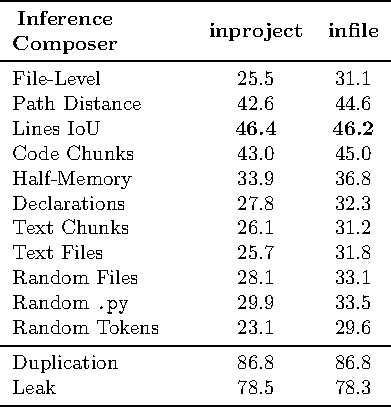
\includegraphics{tables/rq-a1.pdf}
    \caption{Exact Match scores of DeepSeek-Coder-Base 1.3B benchmarked on the LCA}\label{tab:dseek-inference}
\end{table}

A noticeable difference is observed, allowing us to infer that the context provided to the model during inference has a significant impact on its performance. Some detailed findings are as follows:

\begin{enumerate}
\item In-context learning enables the model to leverage any form of meaningful context to improve \textit{infile} completion, indicating that API declarations are not the sole source of metric improvements and that project-level information provides auxiliary grounding for generation.
\item The Lines IoU approach proposes the most effective relevance function for retrieval-augmented generation among the presented methods, demonstrating that the model can achieve the same level of \textit{inproject} performance as \textit{infile}, given the context of sufficient quality.
\item The examination of Declarations indicates that function and class declarations alone do not provide a strong foundation for in-context learning capabilities; the functional code within their bodies is more important.
\item A comparison between Random \texttt{.py} and Text Files suggests that configuration and documentation files are less important for the model than randomly selected code examples in the context. The same observation applies to code comments and documentation strings produced by Text Chunks.
\item Even randomly selected files enhance the code completion capabilities of the model.
\item Random Tokens degrade performance only slightly compared to the File-Level composer, indicating that the model is highly, though not completely, robust to the presence of noisy context.
\item The model is capable of effectively copying (Duplication) and extracting (Leak) ground truth lines from the context without requiring any additional training.
\end{enumerate}

\section{Fine-Tuning on Compositions}\label{sec:fine-tuning-on-compositions}

To estimate the impact of the context composition strategy employed during model fine-tuning, we subject the same model from the previous section to training with various composers. After fine-tuning, we benchmark the model to produce Table~\ref{tab:dseek-fine-tuning}.

\begin{table}[htbp]
    \centering
    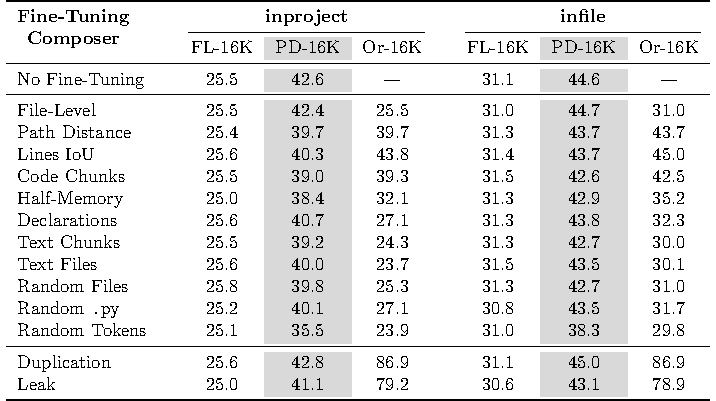
\includegraphics[width=\textwidth]{tables/rq-a2.pdf}
    \caption{Exact Match scores of DeepSeek-Coder-Base 1.3B fine-tuned with different context composition strategies. The rows indicate the composer used to obtain the model checkpoint. The columns represent different evaluation setups: PD for Path Distance, FL for File-Level, and Or for the composer used during fine-tuning. All sequences are truncated to 16K tokens. The blank cells refer to the Table~\ref{tab:dseek-inference}.}\label{tab:dseek-fine-tuning}
\end{table}

The marginal differences in metric values suggest that this particular model is sufficiently trained and is not significantly affected by subsequent fine-tuning.

One might argue that the number of training steps is insufficient. To address this concern, we monitor the learning curves during training and observe that the metric improvements are too small to justify further scaling of this experimental direction. For instance, the best linear slope, \(1.28 \times 10^{-5}\) of EM, is achieved by the Lines IoU composer during the first \(512\) iterations. Applying a linear extrapolation of this slope implies that the model would require more iterations to gain 5 EM points than permitted by the learning rate scheduler. Moreover, since the best model to approximate a learning curve is a logarithmic function, this extrapolation is extremely optimistic.  % TODO: cite scaling laws?

Additionally, we explored different setups to address the issue of the model's robustness to this type of fine-tuning. First, a different training dataset with lower data diversity was used earlier, which resulted in overfitting after the first epoch. Second, we experimented with other hyperparameter choices without success. Third, to eliminate researcher proficiency bias, the experiments were independently reproduced from scratch by another person, which is beyond the scope of this thesis.

\section{Effect of Context Extension}\label{sec:effect-of-context-extension}

We assess the impact of repository-level pre-training on the previously obtained in-context learning capabilities of the model using the composition strategies accessible to OpenCoder-1.5B-Base, which has an original context size limitation of 4K tokens. The summarized results are presented in Table~\ref{tab:ocoder-in-context-retention}. For the extended version, which includes the effects observed with \textit{reversed} and \textit{irrelevant} order modifications, refer to Table~\ref{tab:ocoder-extension-extended}. % TODO: Consider referring to the appendix instead?

\begin{table}[htbp]
    \centering
    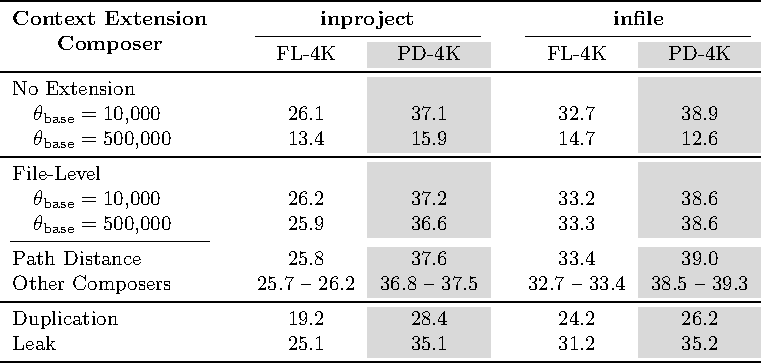
\includegraphics[width=\textwidth]{tables/rq-b1.pdf}
    \caption{Exact Match scores of OpenCoder-1.5B-Base under different evaluation setups. The original model's performance is denoted by No Extension. The other rows represent the checkpoints obtained with the respective composers. Context extension is performed with 4K-token sequences for the File-Level and 16K-token sequences for all other composers. The column notations are consistent with the previous table.}\label{tab:ocoder-in-context-retention}
\end{table}

Three main observations can be drawn from the table to address \hyperref[rq:rq-b1]{RQ.B1}:

\begin{enumerate}
\item ABF without additional fine-tuning significantly impairs the ICL capabilities.
\item The context extension procedure effectively restores model performance after RoPE frequency scaling. Even the File-Level composer, which utilizes input sequences up to 4K tokens, enables the model to adapt to the new \(\theta_{\mathrm{base}}\) value and maintain the same performance level as the original model.
\item Data leakage of ground truth lines impedes the recovery of the model's ICL capabilities. This effect is particularly pronounced for the Duplication composer.
\end{enumerate}

\section{Influence of Composition on Context Extension}\label{sec:influence-of-composition-on-context-extension}

In this section, we address the final research question \hyperref[rq:rq-b2]{RQ.B2} by evaluating the checkpoints obtained after context extension fine-tuning, using various composers to construct the training context. Our conclusions are drawn from Table~\ref{tab:ocoder-extension}, which is a subset of the comprehensive Table~\ref{tab:ocoder-extension-extended}.

\begin{table}[htbp]
    \centering
    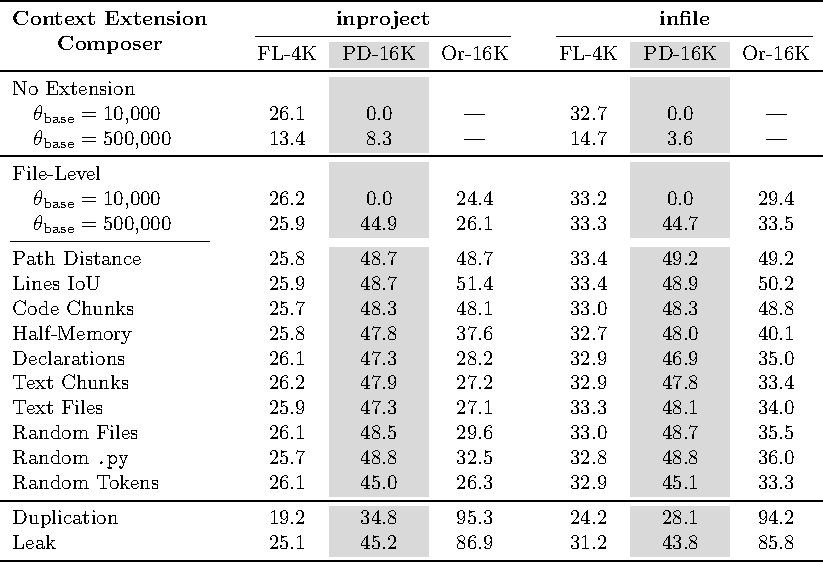
\includegraphics[width=\textwidth]{tables/rq-b2.pdf}
    \caption{Exact Match scores collected from the long-context evaluation of composer choices employed during the repository-level pre-training stage. All clarifying remarks are consistent with the previous table. Blank cells indicate the absence of a repository-level pre-training stage in OpenCoder's development pipeline.}\label{tab:ocoder-extension}
\end{table}

To summarize the outcomes of our study, we present the following observations:

\begin{enumerate}
\item As expected, the original model is unable to utilize the 16K context window. The preliminary base frequency adjustment provides only a negligible improvement and necessitates an additional optimization phase.
\item The context composition strategy employed during the repository-level pre-training stage has only a marginal impact on the final model quality. This finding suggests that adaptation to the RoPE adjustment is the primary driver of long-context improvements.
\item It is possible to significantly reduce computational requirements while still achieving competitive results at the repository-level pre-training stage. For instance, file-level training remains highly effective, even without any repository context and with a context window size limited to 4k tokens.
\item The Duplication composer proves its uncompetitiveness even when compared to the entirely irrelevant context obtained from Random Tokens. This suggests that the data must present at least some degree of challenge to the model in order to foster the development of additional capabilities.
\end{enumerate}

The practical contribution of this research is the identification of a low-resource approach to repository-level pre-training. Context extension fine-tuning can be restricted to the Path Distance composer, requiring only 1B training tokens, while the File-Level presents an even more resource-efficient alternative, necessitating just 73M training tokens. We further demonstrate the utility of this setup by comparing it with DeepSeek-Coder-Base 1.3B, which used 8.4B tokens for repository-level pre-training, and Qwen2.5-Coder-1.5B~\parencite{hui2024}, which employed 300B tokens during the same stage. Figure~\ref{fig:model-comparison} visualizes this comparison, and Figure~\ref{fig:beyond-training-window-inproject} illustrates the performance scaling beyond the training context window for all four models.

\begin{figure}[ht]
    \centering
    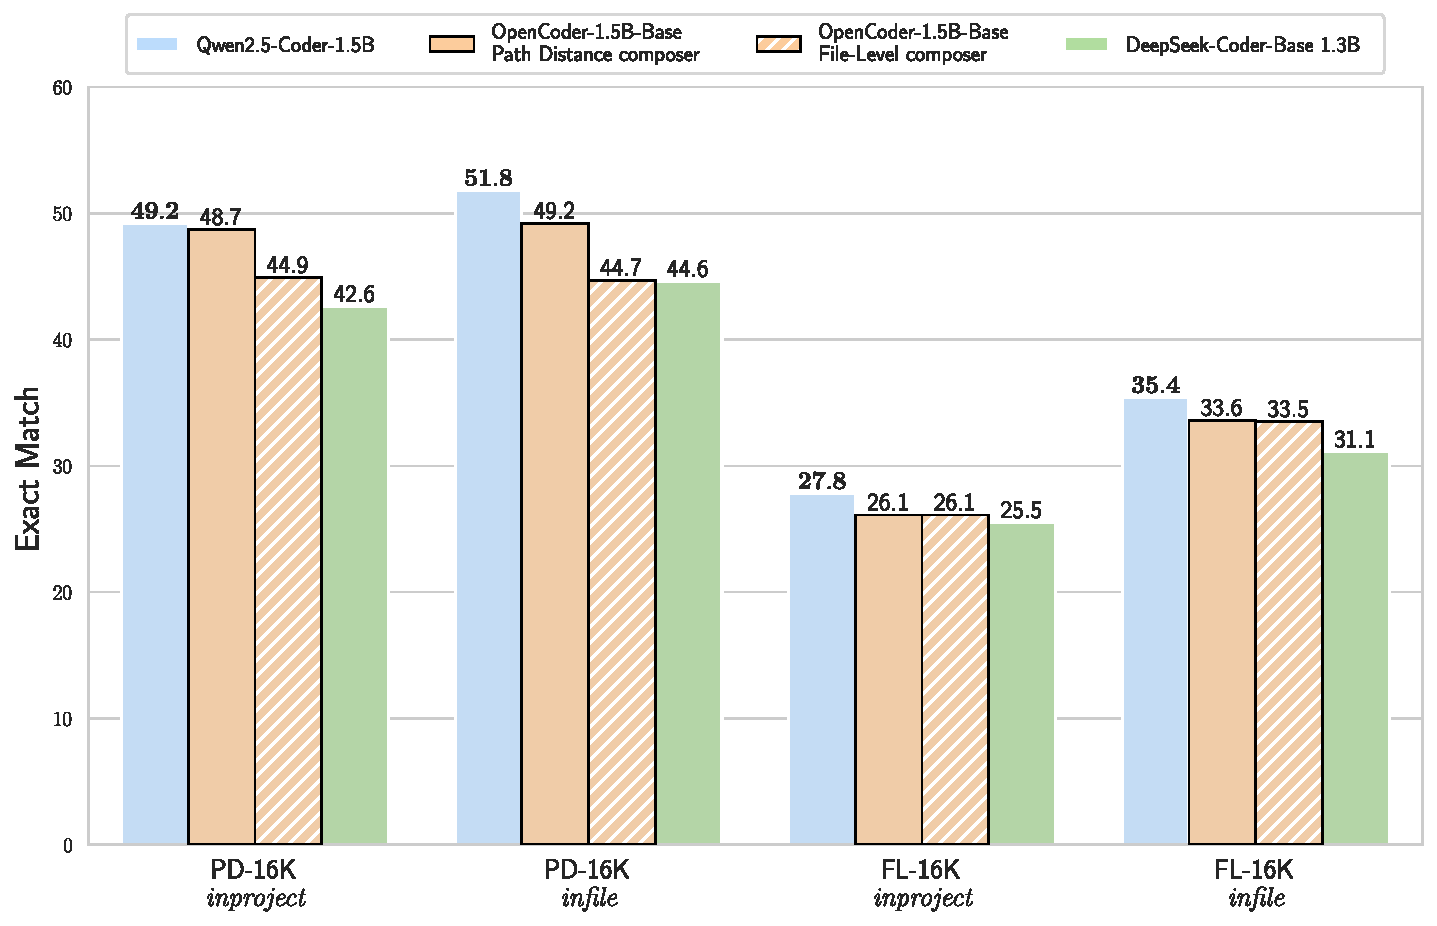
\includegraphics[width=\textwidth]{figures/model-comparison.pdf}
    \caption{Comparison of our two main checkpoints with other existing Code LLMs of the same weight class. The PD-16K setup is used to produce the metric assessment.}\label{fig:model-comparison}
\end{figure}

\begin{figure}[ht]
    \centering
    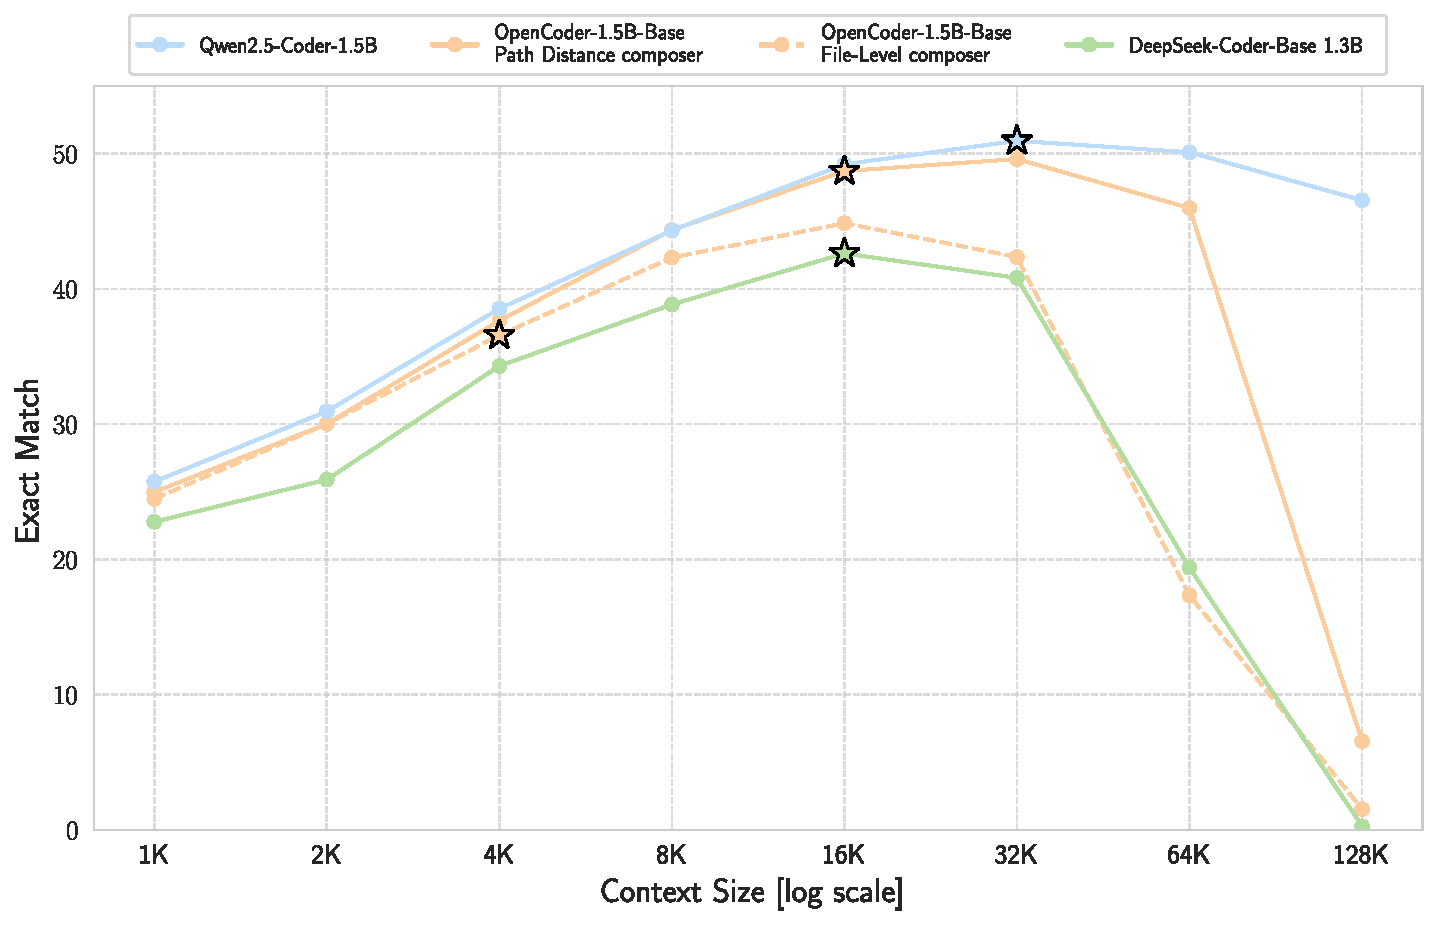
\includegraphics[width=\textwidth]{figures/beyond-training-window-inproject.pdf}
    \caption{Evaluation of the performance 
    scaling beyond the context extension 
    window. The \textit{inproject} line type from the LCA benchmark is selected for visualization; the corresponding Figure~\ref{fig:beyond-training-window-infile} presents results for the \textit{infile} category. ``1K'' refers to 1024 tokens. The \raisebox{-0.3ex}{\FiveStarOpen} markers denote the context length used during repository-level pre-training stage.}\label{fig:beyond-training-window-inproject}
\end{figure}

\todo{Interpretation of the figures}

\section{Supplementary Results}
% TODO: gradient masking
% TODO: use term "inlier" when discussing the gradient masking impact
% TODO: highlight that we extrapolate the results of inlier gradient masking to outlier
% TODO: composer quality analysis:
% api_gain := infile_fl16k
% auxiliary_grounding_gain := infile_or16k - api_gain
% inproject_fl16k + auxiliary_grounding_gain + x * api_gain = inproject_or16k
% x = (inproject_or16k - inproject_fl16k - auxiliary_grounding_gain) / api_gain
% retrieval_quality := x
% retrieval_quality = (inproject_or16k - inproject_fl16k - infile_or16k + infile_fl16k) / infile_fl16k
% iou_quality = 18.6 %
% path_distance_quality = 11.6 %

\section{Limitations and Future Work}
% scale different directions, ...

% TODO: if this section is too small just wrap it as a third paragraph of the conclusion

\chapter*{Conclusion}\addcontentsline{toc}{chapter}{Conclusion}\markboth{Conclusion}{Conclusion}

In conclusion, the objectives of this thesis have been accomplished. The theory of modern repository-level code completion systems is covered in \nameref{part:conceptual-framework}, providing an overview of the code completion task, a general formulation of language modeling, and deep learning methods addressing this area. Subsequently, the specifics of project-level completion are discussed through the lens of language modeling. The relevance and importance of the in-context learning phenomenon are described. To further explore the nuances of repository-level code completion, the general problems of long context are presented along with methods to address them. The research aspect of this work is detailed in \nameref{part:applied-research}, which includes answers to four research questions and a description of the practical framework developed to support these investigations.

The conducted research has yielded several significant findings regarding repository-level code completion. The results substantiate the crucial role of repository context in enhancing completion quality. Contemporary base Code LLMs possess sufficient training, with their in-context learning capabilities showing only marginal improvement through downstream fine-tuning on different context composition strategies. Data leakage in the repository context during the context extension phase adversely affects the model's in-context abilities, while other composers maintain baseline performance integrity. The context composition strategy employed during the repository-level pre-training stage demonstrates minimal impact on final model quality, suggesting that RoPE adjustment serves as the primary driver of long-context improvements and underscores its usage limitations. Additionally, computational requirements of the repository-level pre-training stage can be substantially reduced while maintaining competitive results. For instance, file-level training, even without repository context, remains highly effective. Finally, gradient masking produces a statistically significant yet marginal performance decrease on composers generating inlier context.

Overall, this thesis contributes to the evolution of code completion models by underscoring theoretical foundations in the conceptual framework and offering valuable empirical insights for practitioners through comprehensive research on context composition techniques for repository-level understanding.


\appendix\appendixinit

\chapter{Appendix}

\section{Supplementary Figures and Tables}

\begin{table}[htbp]
    \centering
    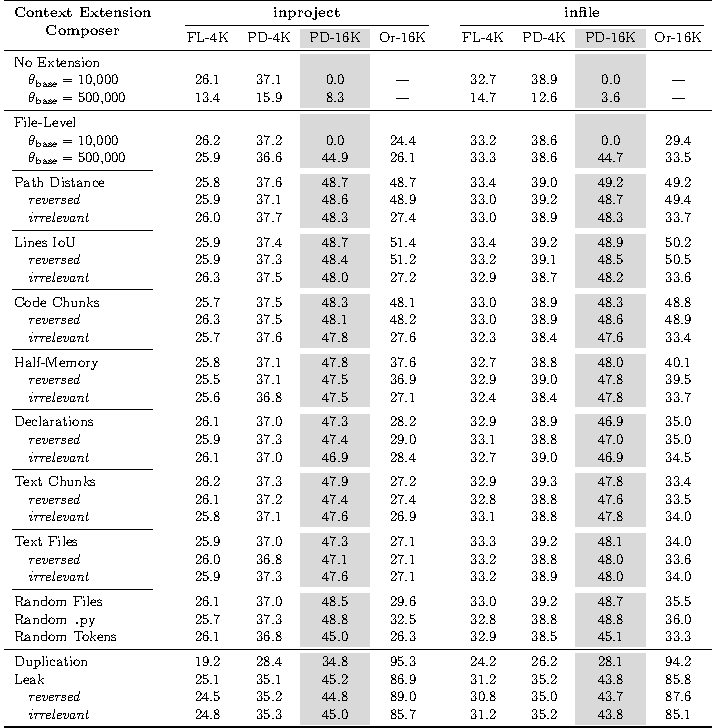
\includegraphics[width=\textwidth]{tables/rq-b.pdf}
    \caption{Extended table presenting the evaluation results for OpenCoder-1.5B-Base, which underwent the repository-level pre-training stage. A more detailed description of the evaluation setup is provided in Section~\ref{sec:evaluation}.}\label{tab:ocoder-extension-extended}
\end{table}

\begin{table}[htbp]
    \centering
    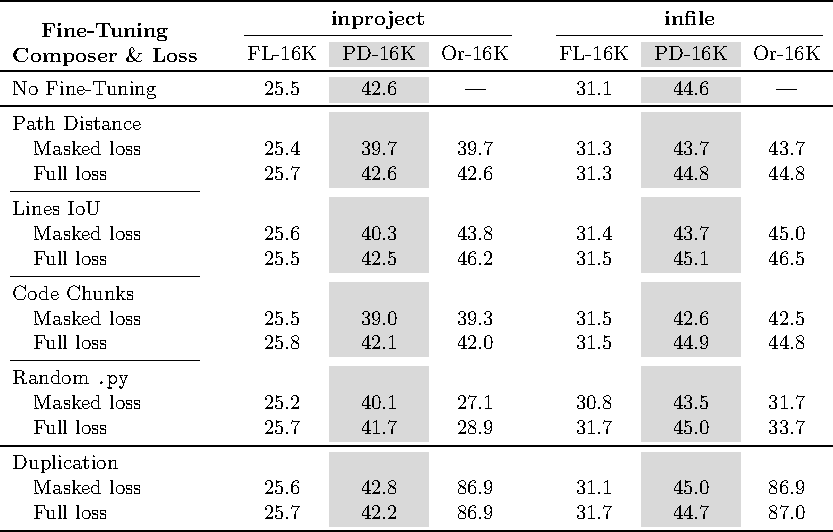
\includegraphics[width=\textwidth]{tables/rq-a2-gradient-masking.pdf}
    \caption{Exact Match scores for DeepSeek-Coder-Base 1.3B fine-tuned on composers generating inlier repository context for the completion file under two training setups: with and without gradient masking}\label{tab:dseek-gradient-masking}
\end{table}

\begin{table}[htbp]
    \centering
    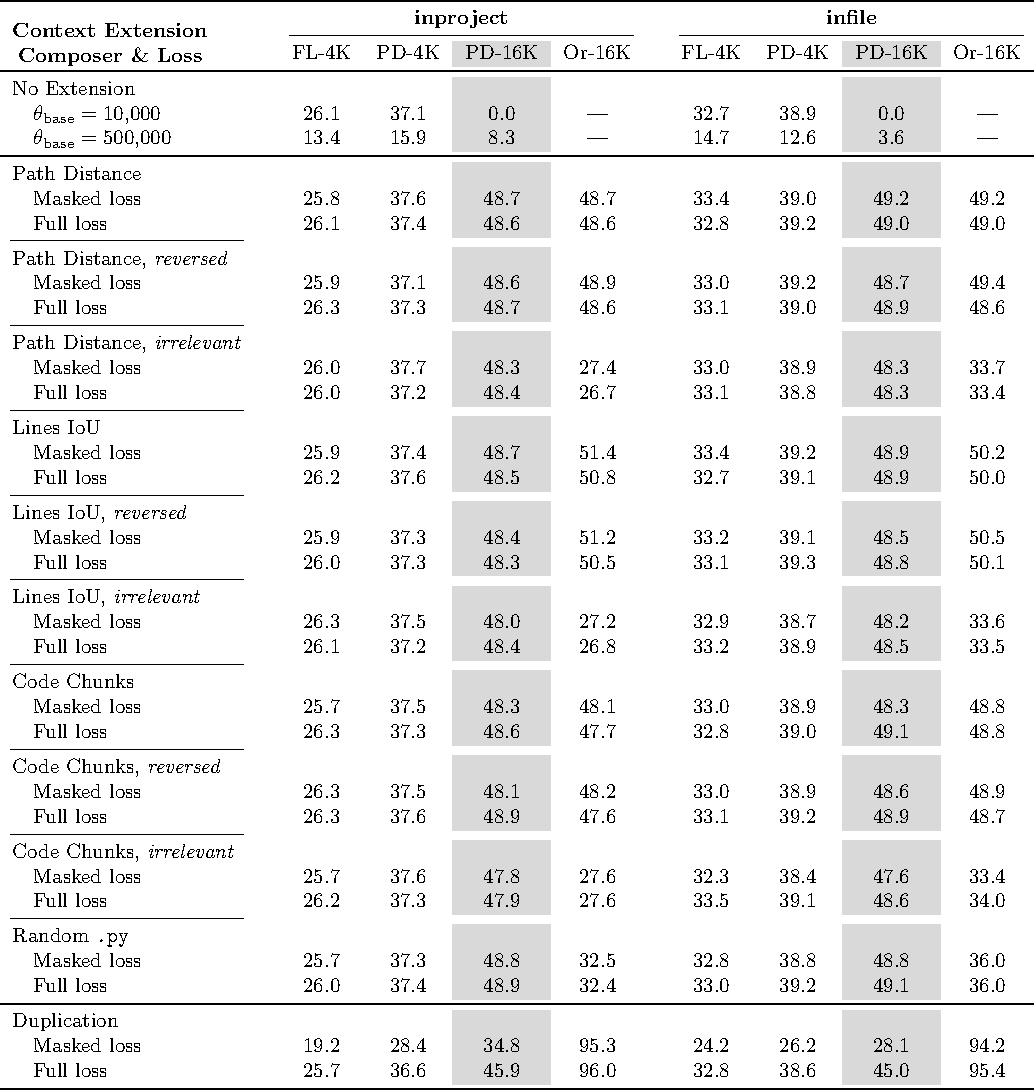
\includegraphics[width=\textwidth]{tables/rq-b-gradient-masking.pdf}
    \caption{Exact Match scores for repository-level pre-trained OpenCoder-1.5B-Base on composers generating inlier repository context for the completion file under two training setups: with and without gradient masking}\label{tab:ocoder-gradient-masking}
\end{table}

\begin{figure}[ht]
    \centering
    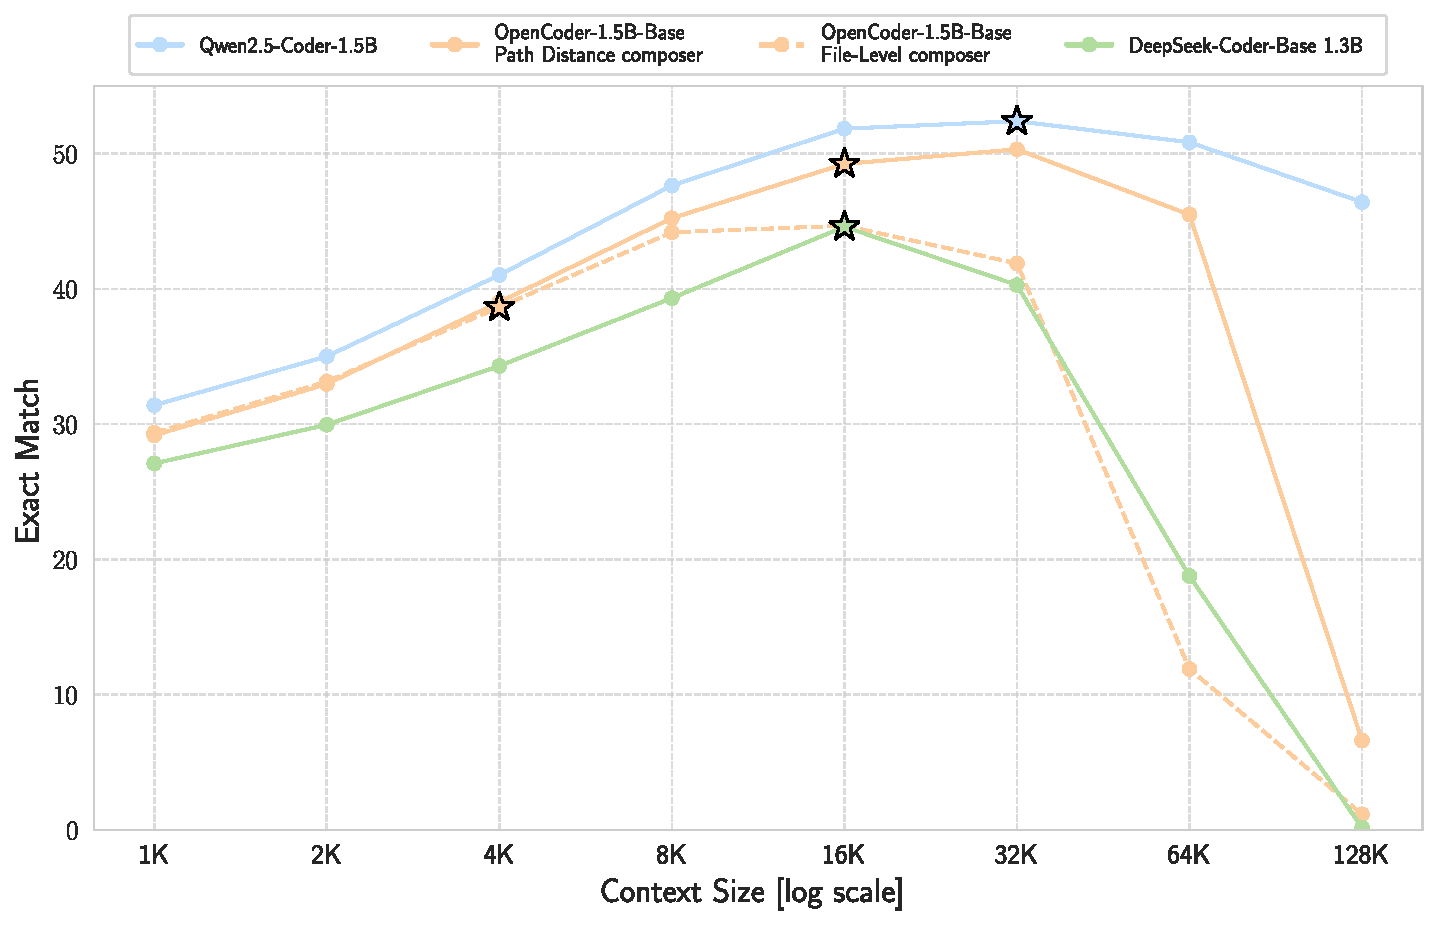
\includegraphics[width=\textwidth]{figures/beyond-training-window-infile.pdf}
    \caption{Evaluation of the performance scaling beyond the context extension window. The \textit{infile} line type from the LCA benchmark is selected for visualization; the corresponding Figure~\ref{fig:beyond-training-window-inproject} presents results for the \textit{inproject} category. ``1K'' refers to 1,024 tokens. The \raisebox{-0.3ex}{\FiveStarOpen} markers denote the context length used during repository-level pre-training stage.}\label{fig:beyond-training-window-infile}
\end{figure}


\backmatter

\chapter*{Bibliography}
% Split bibliography with sapronov2025 first, then a gap, then all other references
\setlength{\emergencystretch}{\textwidth}
\printbibliography[category=our_papers,heading=none]
\printbibliography[notcategory=our_papers,heading=none]

\chapter{Contents of the attachment}

Not ready.

	% TODO: fill in the contents of the attachment (irrelevant example is provided)
	% \dirtree{%
	% 	.1 /.
	% 	.2 readme.txt\DTcomment{short description of the media}.
	% 	.2 exe\DTcomment{directory with the executable form of the implementation}.
	% 	.2 src.
	% 	.3 impl\DTcomment{source codes of the implementation}.
	% 		.3 thesis\DTcomment{zdrojová forma práce ve formátu \LaTeX{}}.
	% 		.2 text\DTcomment{text práce}.
	% 		.3 thesis.pdf\DTcomment{text práce ve formátu PDF}.
	% }
 % include `medium.tex' from `text/' subdirectory

\end{document}
